 \documentclass[lettersize,journal]{IEEEtran}
\usepackage{amsmath,amsfonts}
\usepackage{algorithmic}
\usepackage{algorithm}
\usepackage{array}
\usepackage[caption=false,font=footnotesize,labelfont=rm,textfont=rm]{subfig}
\usepackage{textcomp}
\usepackage{stfloats}
\usepackage{url}
\usepackage{verbatim}
\usepackage{graphicx}
\usepackage{cite}
\usepackage{booktabs}
\usepackage{multirow}
\usepackage{color}
\usepackage{xcolor}
\usepackage{soul} 
\usepackage{tcolorbox}
\sethlcolor{red}
\soulregister{\cite}7 % 注册\cite命令
\soulregister{\citep}7 % 注册\citep命令
\soulregister{\citet}7 % 注册\citet命令
\soulregister{\ref}7 % 注册\ref命令
\soulregister{\pageref}7 % 注册\pageref命令
\usepackage[table]{xcolor}


\hyphenation{op-tical net-works semi-conduc-tor IEEE-Xplore}
% updated with editorial comments 8/9/2021

\begin{document}

\title{WaveLoop: Recurrent Wavelet Network for Video Crowd Counting}

\author{Junyu Sun, Miaogen Ling, Wei Fang and Xin Geng,~\IEEEmembership{Senior Member,~IEEE}
        % <-this % stops a space
% \thanks{This paper was produced by the IEEE Publication Technology Group. They are in Piscataway, NJ.}% <-this % stops a space
\thanks{Manuscript received **; revised **. This research is supported by the Jiangsu Science Foundation (BG2024036, BK20243012), the National Science Foundation of China (62202235, 62125602, U24A20324, 92464301), the New Cornerstone Science Foundation through the XPLORER PRIZE, and the Fundamental Research Funds for the Central Universities (2242025K30024). \textit{(Corresponding author: Xin Geng.)}}
\thanks{Miaogen Ling is with the School of Computer Science, Nanjing University of Information Science and Technology, Nanjing 210044, China, and also with the Provincial Key Laboratory for Computer Information Processing Technology, Soochow University, Suzhou 215006, China (e-mail: mgling@nuist.edu.cn).}
\thanks{Junyu Sun and Wei Fang are with the School of Computer Science, Nanjing University of Information Science and Technology, Nanjing 210044, China (e-mail: 202412492179@nuist.edu.cn; fangwei@nuist.edu.cn).}
\thanks{Xin Geng is with the School of Computer Science and Engineering, Southeast University, Nanjing 211189, China (e-mail: xgeng@seu.edu.cn).}
\thanks{Copyright © 2026 IEEE. Personal use of this material is permitted. However, permission to use this material for any other purposes must be obtained from the IEEE by sending an email to pubs-permissions@ieee.org.}
}

% The paper headers
\markboth{IEEE Transactions On Circuits and Systems For Video Technology}%
{Shell \MakeLowercase{\textit{et al.}}: A Sample Article Using IEEEtran.cls for IEEE Journals}

% \IEEEpubid{0000--0000/00\$00.00~\copyright~2021 IEEE}
% Remember, if you use this you must call \IEEEpubidadjcol in the second
% column for its text to clear the IEEEpubid mark.

\maketitle

\begin{abstract}
Video crowd counting exploits temporal information from consecutive frames to improve density estimation. However, existing methods either require costly multi-frame modeling or rely on explicit motion cues that mainly capture rapid inter-frame changes. Moreover, independently estimating each frame limits temporal consistency, while the semantic discrepancy between spatial and frequency representations hinders effective feature interaction. To address these issues, we propose WaveLoop, a recurrent wavelet network for video crowd counting. WaveLoop applies spatial discrete wavelet transform to extract complementary frequency components and introduces a Scale-Aligned Frequency Fusion module to alleviate the magnitude discrepancy between low- and high-frequency sub-bands. Temporal discrete wavelet transform is further employed to separate slowly varying crowd trends from rapid temporal variations, which are exploited by a Temporal Frequency Reconfiguration Module to adaptively modulate single-frame frequency features. Meanwhile, a Density-Guided Frequency Attention module utilizes density-aware spatial priors to enhance frequency representations, and a Dual-Domain Similarity Enhancement module reinforces semantically consistent regions during feature fusion. Historical density predictions are recurrently propagated across frames, together with a temporal consistency loss, to improve long-term temporal modeling and prediction stability. Extensive experiments on five benchmark datasets demonstrate that WaveLoop achieves state-of-the-art performance. On the Classroom dataset, WaveLoop 
achieves 8.5\%/9.9\% improvements in MAE/RMSE over the best existing  method. The code is available at: https://...
\end{abstract}



\begin{IEEEkeywords}
Video crowd counting, Temporal-frequency modeling, Discrete wavelet transform, Frame-recurrent learning, Cross-domain interaction.
\end{IEEEkeywords}




\section{Introduction}
\label{Intro}
\IEEEPARstart{C}{rowd} counting has become an increasingly important task in computer vision due to its wide range of applications in intelligent surveillance, public safety monitoring, traffic management, and urban planning. Compared with image-based crowd counting, video crowd counting aims to estimate crowd density by leveraging both spatial appearance and temporal dynamics from consecutive frames. The additional temporal information provides valuable cues for modeling crowd motion and improving estimation robustness. Nevertheless, accurately counting people in complex video scenes remains challenging due to factors such as severe occlusion, motion ambiguity and illumination changes. Addressing these challenges is essential for developing reliable video crowd counting systems in real-world environments.


Previous video crowd counting methods can be roughly classified into two categories: spatiotemporal modeling methods and motion-guided methods. The spatiotemporal modeling methods \cite{xiong2017spatiotemporal,zou2019enhanced,ma2021spatiotemporal,dong2022clrnet,cai2022global,wu2022spatial,ling2025dual,ling2026dual,ling2026cascaded} 
typically utilize consecutive video frames to capture temporal dynamics and generate density maps by modeling inter-frame dependencies.
Existing methods commonly employ a spatial backbone to extract features and further introduce temporal interaction modules to model dependencies across consecutive frames. However, these approaches generally require multiple consecutive frames to capture long-range temporal dependencies, which inevitably incurs additional computational overhead. Furthermore, density maps are typically estimated independently for each frame, with limited interaction among consecutive predictions.

The second category leverages explicit motion cues, such as optical flow\cite{ranjan2017optical,hossain2020video,hou2023frame,cao2024efficient} or frame differences\cite{ling2023motional}, to facilitate crowd dynamics modeling and improve density estimation. However, these methods mainly rely on explicit motion cues to model temporal dependencies, which primarily capture rapid motion changes between adjacent frames while paying less attention to the underlying temporal evolution of crowd scenes. As a result, their ability to comprehensively capture complex crowd dynamics remains limited.


Although existing methods are effective to a certain extent, they  still  suffer from three problems. First, motion-guided approaches mainly rely on rapid motion cues for temporal modeling, may overlook complementary temporal patterns such as slowly varying crowd trends. Second, integrating useful information from different domains remains challenging because of their semantic discrepancy, existing methods usually require additional alignment or fusion operations to bridge this gap. Third, many existing methods estimate the density map of each frame independently, without explicitly modeling interactions among density predictions across adjacent frames, resulting in limited temporal consistency.
%Finally, most existing methods rely on multiple consecutive frames to capture long-range temporal dependencies and often require future frame information, which limits their applicability in real-world deployment.

Motivated by these observations, we propose a Recurrent Wavelet Network (WaveLoop) to model crowd dynamics through temporal frequency-domain representations with spatial guidance for video crowd counting. Instead of explicitly extracting motion information through optical flow or frame differencing, we employ the Temporal Discrete Wavelet Transform (DWT-T) to decompose a two-frame video sequence into one temporal high-frequency sub-band and one temporal low-frequency sub-band. As shown in Fig.~\ref{fig:1}(A), the Spatial Discrete Wavelet Transform (DWT-S) can decompose an image into one low frequency sub-band and three 
high frequency sub-bands of different directions (horizontal, vertical, diagonal). Fig.~\ref{fig:1}(B) shows the Temporal Discrete Wavelet Transform (DWT-T), the temporal high-frequency component captures rapid temporal variations and details, reflecting how crowd patterns change over time, whereas the temporal low-frequency component preserves slowly varying temporal trends that describe the overall evolution of the crowd. By modeling these complementary frequency components, our framework is able to simultaneously capture slowly varying crowd trends and rapidly changing motion details. These temporal representations are then utilized to modulate single-frame features, allowing the model to exploit richer temporal context and learn more robust feature representations. Thus, the first limitation is solved by using discrete wavelet transform in temporal dimension.

Subsequently, we solve the second problem by introducing the density-guided frequency attention (DGFA) module. Specifically, spatial features are utilized as auxiliary guidance to facilitate information exchange with frequency representations through cross-attention. Furthermore, spatial features are leveraged to estimate a density map, whose density-related cues are subsequently encoded by a lightweight temperature predictor to generate adaptive attention temperatures. This design allows the attention mechanism to dynamically adjust its focus according to crowd density distributions, facilitating more effective cross-domain feature aggregation. In this way, frequency representations can be effectively enhanced through spatial guidance without requiring explicit feature alignment.

To address the third problem, we employ a recurrent propagation mechanism that takes the previously estimated density map as an additional input for subsequent prediction. In this manner, temporal information can be progressively accumulated across frames, enabling long-term temporal modeling without relying on fixed-length frame sequences. Moreover, a temporal consistency loss (TCL) is introduced to explicitly constrain the variation between consecutive density maps. Specifically, the difference between adjacent predicted density maps is supervised by the corresponding difference between ground-truth density maps using an L1 loss. As a result, the proposed framework not only produces temporally consistent density estimations but also facilitates practical online deployment by eliminating the dependency on future-frame information.


The main contributions of this study are listed as follows:
\begin{itemize}
    \item  We propose WaveLoop, a frame-recurrent wavelet network for video crowd counting. It recurrently propagates historical density predictions and introduces a temporal consistency constraint to improve prediction stability across consecutive frames.

    \item  We introduce a scale-aligned frequency fusion (SAFF) module to alleviate the magnitude discrepancy between spatial low- and high-frequency components, and a temporal frequency reconfiguration module (TFRM) to inject temporal information into single-frame frequency features.

    \item We develop a density-guided frequency attention (DGFA) module to enhance frequency representations using density-aware spatial priors. A dual-domain similarity enhancement (DSE) module is further designed to reinforce consistent regions between temporal-frequency and frequency-spatial representations.

    \item  The proposed WaveLoop achieves state-of-the-art performance on five benchmark datasets. Specifically, it surpasses the second-best method by 8.5\% in MAE and 9.9\% in RMSE on the Classroom dataset.

\end{itemize}

\begin{figure}[h]
 \centering  
 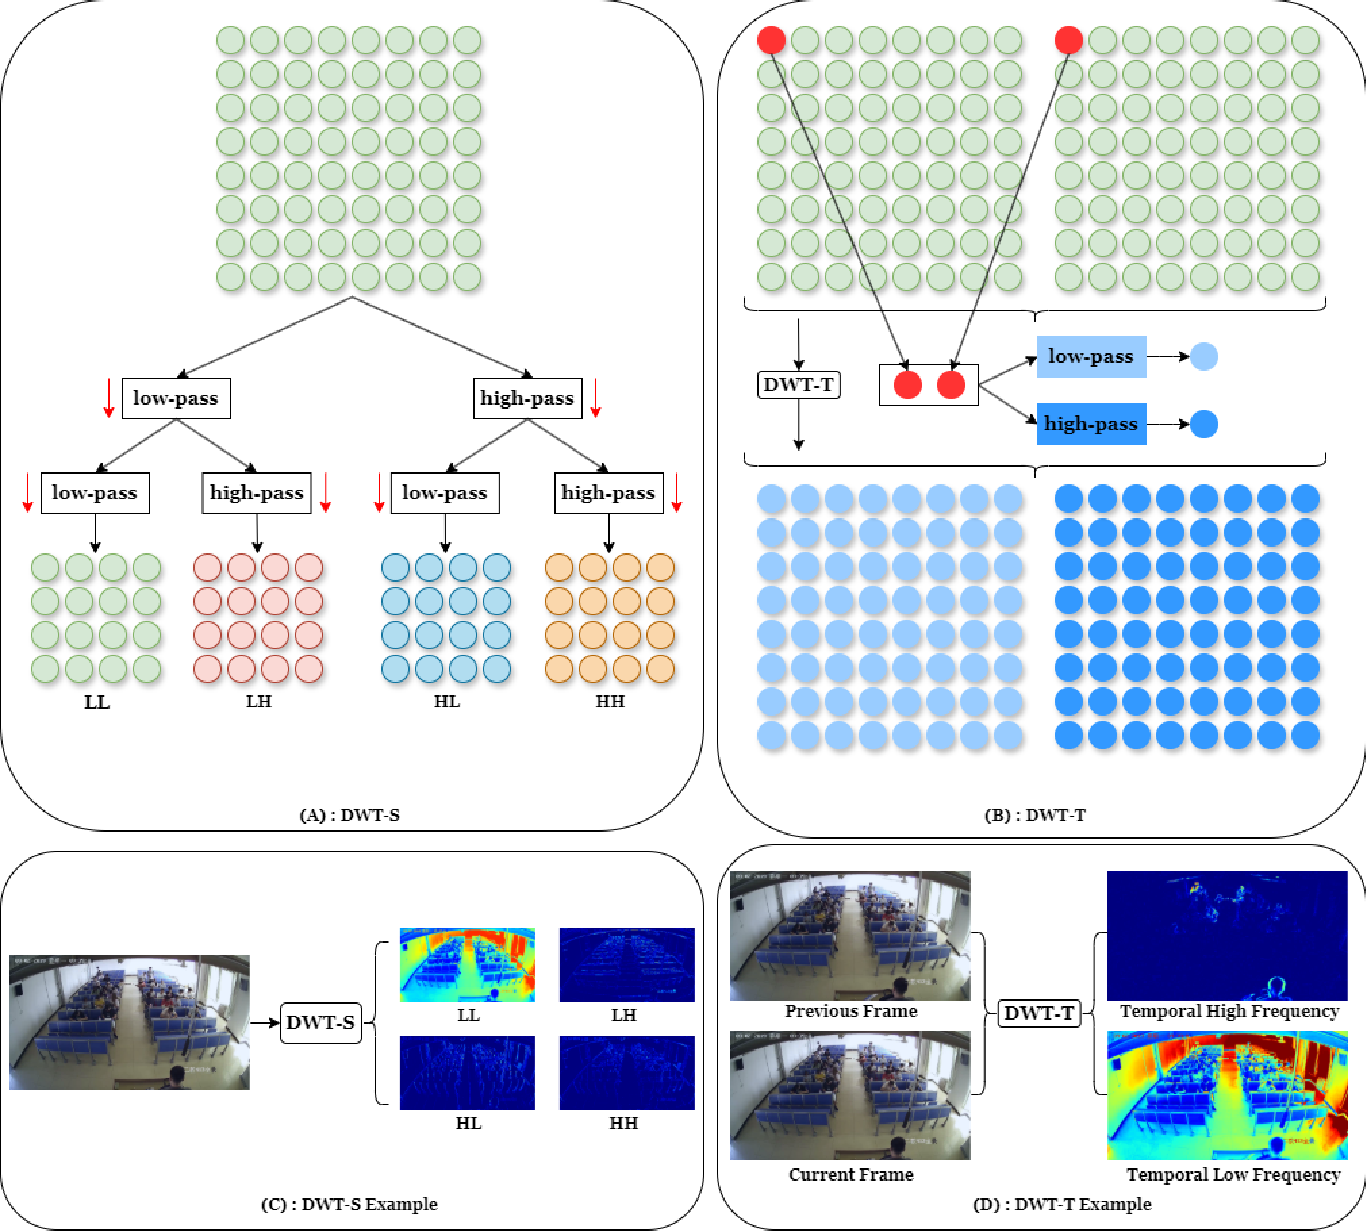
\includegraphics[width=0.47\textwidth]{Example.pdf}
    \caption{(A): Spatial Discrete Wavelet Transform (DWT-S) decomposes an image into one low-frequency sub-band (LL) and three high-frequency sub-bands (LH, HL, and HH), where the high-frequency sub-bands capture horizontal, vertical, and diagonal directions, respectively. (B): Discrete Wavelet Transform in temporal dimension (DWT-T) decomposes an image sequence into a temporal low-frequency sub-band and a temporal high-frequency sub-band along the temporal axis. (C): A visualization example of DWT-S, The sub-bands are visualized in heatmap style. (D): A visualization example of DWT-T.}
\label{fig:1}
\vspace{-0.5em}
\end{figure}

\section{Related Work}
\subsection{Single Image Crowd Counting}
Single-image crowd counting has been extensively studied over the past decade. Early studies explored crowd estimation through pedestrian detection \cite{ge2009marked,dollar2011pedestrian} and point localization \cite{song2021rethinking,liang2022focal,liu2023point,chen2024improving}. However, these methods often struggle in highly congested scenes due to severe occlusions and complex crowd distributions. Currently, density map estimation has become the dominant paradigm for crowd counting. Density map-based methods \cite{sindagi2017generating, chen2019scale,yang2020embedding,jiang2020attention,yan2021towards,liu2022lw,lin2022boosting,lin2024gramformer} estimate crowd counts by predicting a density map and summing its values to obtain the total number of people. Early density estimation approaches mainly addressed the scale variation problem in crowded scenes through multi-scale feature extraction. For example, multi-scale approaches \cite{sindagi2017generating, chen2019scale} propose pyramid networks to capture crowd patterns at diverse scales. With the advancement of attention mechanisms, recent methods have achieved more discriminative feature representations for crowd density estimation. For instance, Jiang et al.\cite{jiang2020attention} employ density-aware attention to adaptively reweight regions with different crowd densities. Lin et al.\cite{lin2022boosting} propose MAN to adaptively emphasize informative regions. Similarly, Lin et al.\cite{lin2024gramformer} enhance both attention modeling and input feature learning, enabling more discriminative crowd feature representations. Despite their success, these approaches estimate each frame independently and fail to exploit temporal cues available in video sequences.
%MCNN\cite{haq2023mcnn} employ multiple convolutional branches with different receptive fields to capture crowd patterns at diverse scales. With the development of attention mechanisms, lin2024gramformer



\subsection{Video Crowd Counting}
Compared with single-image crowd counting methods, video crowd counting methods leverage temporal dependencies across consecutive frames to obtain more accurate and temporally consistent crowd estimations. Recent studies can be categorized into spatiotemporal modeling methods and motion-guided methods. Spatiotemporal modeling methods\cite{xiong2017spatiotemporal,zou2019enhanced,ma2021spatiotemporal,wu2022spatial,cai2022global,dong2022clrnet,ling2025dual,ling2026dual,ling2026cascaded} utilize a sequence of adjacent frames to learn both spatial representations and temporal dependencies. Some studies \cite{zou2019enhanced,ma2021spatiotemporal,ling2026dual} employ 3D convolutions\cite{tran2015learning} to capture spatial and temporal dependencies from consecutive video frames. For example, Ling et al.\cite{ling2026dual} extend pretrained spatial representations to the temporal domain through 3D convolutional operations. However, 3D convolutions usually introduce substantial computational and memory overhead due to the additional temporal dimension. With the success of attention mechanisms\cite{vaswani2017attention}, some studies\cite{wu2022spatial,dong2022clrnet,ling2026cascaded} have leveraged attention-based architectures to better capture temporal dependencies and long-range interactions. For instance, Dong et al.\cite{dong2022clrnet} introduce a pixel-level attention mechanism to model local dependencies across consecutive frames. Ling et al.\cite{ling2026cascaded} introduce an efficient temporal attention mechanism that leverages neighboring frames to dynamically modulate channel-wise feature representations of the current frame.

The second category utilizes motion information to distinguish foreground regions from the background, thereby facilitating more accurate crowd estimation. Some studies\cite{ranjan2017optical,hossain2020video,hou2023frame,cao2024efficient} leverage optical flow as an auxiliary motion cue to enhance temporal feature learning and crowd density estimation. For example, Hou et al.~\cite{hou2023frame} employ optical flow to estimate motion between consecutive frames and fuse historical density information in a frame-recurrent manner. In contrast, Cao et al.~\cite{cao2024efficient} utilize optical flow for temporal collaborative fusion to align adjacent-frame features and derive density residuals, thereby enhancing the counting accuracy of the current frame. Despite their effectiveness, optical flow-based methods usually rely on an additional motion estimation network, leading to increased computational cost. To avoid the computational burden of optical flow estimation, Ling et al.~\cite{ling2023motional} utilize frame differences to generate motion foreground maps, which provide motion-aware cues for crowd density estimation. 

However, both optical flow and frame difference-based methods primarily focus on explicit motion cues and may overlook the complementary temporal patterns in crowd videos, such as slowly evolving crowd trends and rapidly changing motion details. In contrast, our approach employs discrete wavelet transform in the temporal dimension (DWT-T) to decompose a two-frame sequence into temporal low-frequency and high-frequency components, which respectively represent slowly varying crowd trends and rapidly changing motion details. Building upon these complementary temporal-frequency cues, we further propose a Temporal Frequency Reconfiguration Module (TFRM) to inject temporal information into single-frame feature representations.

\subsection{Discrete Wavelet Transform}
Discrete wavelet transform has been widely applied in image processing for its efficient multi-resolution representation and fast implementation via filter banks. The filter bank implementation of wavelets can be viewed as computing wavelet coefficients of a set of child wavelets generated from a given mother wavelet. According to \cite{mallat1989theory}, we illustrate the DWT process along both the spatial dimension of an image and the temporal dimension of a video sequence in Fig.~\ref{fig:1}. Many studies have applied DWT along the spatial dimension for image representation and feature enhancement, such as Yang et al.\cite{yang2024sffnet} introduce a spatial-frequency fusion strategy by decomposing features into frequency components for segmentation. Garg et al.~\cite{garg2024gestformer}  incorporate multi-scale wavelet pooling into Transformer architectures for gesture recognition. Furthermore, Zhang et al.\cite{zhang2024wtvi} design a wavelet-based Transformer for video inpainting, which decomposes video frames into frequency components and employs Transformers for content restoration in the frequency domain.

Beyond spatial decomposition, DWT has also been explored along the temporal dimension of video sequences to model motion-related frequency variations. Jin et al.\cite{jin2020exploring} propose a spatial-temporal multi-frequency analysis framework for video prediction, where temporal DWT operates along the time axis to capture multi-frequency motions and improve temporal consistency. In video coding, Lanz et al.~\cite{lanz2019content} introduce a content-adaptive wavelet lifting scheme that filters video sequences along the temporal axis and decomposes them into low-pass and high-pass temporal sub-bands. Meyer et al.~\cite{meyer2023learned} further develop an end-to-end learnable wavelet video coder based on motion-compensated temporal filtering. These works demonstrate the effectiveness of temporal wavelet decomposition in separating complementary temporal components in video signals. In our approach, we jointly incorporate spatial discrete wavelet decomposition (DWT-S) and discrete wavelet decomposition in temporal dimension (DWT-T) to fully exploit frequency information in both spatial and temporal domains, achieving state-of-the-art performance in crowd counting.

\section{Method}
\subsection{Architecture Overview}
\label{Waveloop}
As illustrated in Fig.~\ref{fig:2}, the proposed WaveLoop adopts a frame-recurrent architecture for video crowd counting. At each time step, the network takes two consecutive frames as the input, denoted as \(Z\in\mathbb{R}^{B\times T\times C\times H\times W}\), where \(B\) denotes the batch size, \(T=2\) is the number of input frames, \(C\) represents the number of channels, and \(H\) and \(W\) denote the frame height and width, respectively. Frequency components obtained by DWT-S are first aggregated by the proposed scale-aligned frequency fusion (SAFF) module and then encoded by the backbone network to obtain single-frame frequency features. Temporal-frequency representations generated by DWT-T are then exploited by the temporal frequency reconfiguration module (TFRM) to modulate these frequency features. Meanwhile, the density-guided frequency attention (DGFA) module enhances the single-frame frequency features under the guidance of spatial features. The outputs of TFRM and DGFA are integrated by the proposed dual-domain similarity enhancement (DSE) module. The fused features are subsequently upsampled by a factor of 2 and fed into the next scale for further refinement following the same procedure. Finally, the refined features are fed into the density estimation head to generate the density map. The predicted density map is then propagated to the next time step, where the above process is repeated for recurrent density estimation.


%As is stated before, most existing video crowd counting methods either rely on multiple consecutive frames to capture long-range temporal dependencies, or focus on rapid motion changes between adjacent frames while overlooking slowly varying crowd evolution trends. In this paper, we propose a recurrent wavelet network (WaveLoop) for video crowd counting.  We take the current frame and previous frame as the inputs to the network. They are denoted as $Z \in \mathbb{R}^{B \times T \times C \times H \times W}$, where $B$ denotes the batch size, $T=2$ is the number of input frames, $C$ represents the number of channels, and $H$ and $W$ denote the height and width of the frames, respectively. First, we apply the spatial discrete wavelet transform (DWT-S) to the current frame to decompose it into one low-frequency sub-band and three high-frequency sub-bands. To fully exploit the complementary advantages of low-frequency structural information and high-frequency detail information, these frequency components are then fed into the scale-aligned frequency fusion (SAFF) module to obtain a fused single-frame frequency representation $F_{in}$. Subsequently, $F_{in}$ and the original frame are fed into a shared ConvNeXt-T \cite{liu2022convnet} backbone network for multi-scale feature extraction, producing single-frame frequency-domain feature maps $F_4$ and spatial-domain feature maps $\{S_3, S_4\}$ at the third and fourth stages, respectively.
%To capture temporal information, we further apply the discrete wavelet transform in time dimension (DWT-T) to two consecutive frames, yielding one temporal low-frequency and one temporal high-frequency component. To emphasize motion magnitude while suppressing sign ambiguity, the temporal high-frequency component is transformed by an absolute value operation. Subsequently, the temporal high-frequency and low-frequency components are fed into two independent lightweight ConvNeXt-Atto \cite{woo2023convnext} backbones for temporal feature encoding. To align the channel dimensions with the third- and fourth-stage outputs of ConvNeXt-T for subsequent interaction, the outputs of the third and fourth stages are projected via $1\times1$ convolutions for channel alignment, yielding temporal low-frequency features $\{TL_3, TL_4\}$ and temporal high-frequency features $\{TH_3, TH_4\}$.
%At the scale of $\frac{H}{32} \times \frac{W}{32}$, the temporal frequency reconfiguration module (TFRM) utilizes $TL_4$ and $TH_4$ to modulate the single-frame frequency feature $F_4$, thereby injecting temporal information into the single-frame frequency representation. Meanwhile, the density-guided frequency attention (DGFA) module employs the spatial feature $S_4$ as auxiliary guidance to perform cross-attention with $F_4$, enhancing the frequency representation with density-aware spatial cues. The outputs of TFRM and DGFA are denoted as $F_4^{T}$ and $F_4^{S}$, respectively. Subsequently, $F_4^{T}$ and $F_4^{S}$ are fed into the dual-domain similarity enhancement (DSE) module and the resulting feature $F_4^{C}$ is then projected and upsampled via bilinear interpolation to obtain $\hat{F}_3$ at the resolution of $\frac{H}{16}\times\frac{W}{16}$. The upsampled feature $\hat{F}_3$ is subsequently processed at the $\frac{H}{16}\times\frac{W}{16}$ scale following the same procedure. Finally, the refined feature is further projected and upsampled to a higher spatial resolution and fed into a regression head to generate the crowd density map of current frame.


\begin{figure*}[t]
  \centering  
  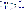
\includegraphics[width=1.0\textwidth]{fw1}
  \caption{Overview of the proposed WaveLoop network. $\vert\cdot\vert$ denotes the absolute value operation. Proj consists of a $1\times1$ convolution, LayerNorm, and GELU. Up denotes bilinear interpolation.}
  \label{fig:2}
  \vspace{-1em}
\end{figure*}



    
\vspace{-0.5em}
\subsection{Scale-Aligned Frequency Fusion} \label{saff}
As described in Sec \ref{Intro}, Spatial Discrete Wavelet Transform (DWT-S) can decompose an image into one low-frequency sub-band ($LL$) and three high-frequency sub-bands ($LH$, $HL$, and $HH$). 
FreqFusion \cite{chen2024frequency} demonstrates that high-frequency components can serve as complementary details to compensate for information loss during feature aggregation. However, the low-frequency and high-frequency components exhibit substantially different statistical distributions and value ranges. A simple aggregation may cause the high-frequency components to either dominate the low-frequency representation or contribute negligibly, thereby limiting effective interaction and fusion between frequency-domain features. Inspired by this, we introduce a scale-aligned frequency fusion (SAFF) module, the high-frequency representation is adaptively rescaled to align its magnitude with that of the low-frequency ($LL$) component before feature aggregation.

Specifically, taking the current frame for example, the three high-frequency sub-bands (\(LH, HL, HH \in \mathbb{R}^{B \times 3 \times \frac{H}{2} \times \frac{W}{2}}\)) are first concatenated along the channel dimension and compressed into a unified high-frequency representation $Y \in\mathbb{R}^{B \times 3 \times \frac{H}{2} \times \frac{W}{2}}$ using a 1×1 convolution. Subsequently, both the low-frequency component \(LL\in\mathbb{R}^{B \times 3 \times \frac{H}{2} \times \frac{W}{2}}\) and the unified high-frequency representation \(Y\) are upsampled to the original spatial resolution via bilinear interpolation, producing the aligned low- and high-frequency representations \(L\) and \(H\), respectively.

Then, to reduce the magnitude discrepancy between frequency bands, we introduce a frequency-band scaling strategy. Specifically, the ratio between the channel-wise standard deviations of  \(L\) and \(H\) is used to derive a scaling factor $Scale$, which can adjust the value range of the high-frequency components and facilitate subsequent feature interaction:
\begin{equation}
\mathbf{Scale}
=
\frac{
\max\!\big(
\mathrm{Std}_{h,w}(\mathbf{L}),
\varepsilon
\big)
}{
\max\!\big(
\mathrm{Std}_{h,w}(\mathbf{H}),
\varepsilon
\big)
},
\qquad
\mathbf{Scale}
\in
\mathbb{R}^{B\times 3\times1\times1}.
\label{eq:scale}
\end{equation}
where $\mathrm{Std}_{h,w}(\cdot)$ denotes the channel-wise standard deviation, and $\varepsilon$ is a small constant introduced to avoid numerical instability caused by division by zero.

Subsequently, the scaled high-frequency feature is fused with the low-frequency representation through a residual aggregation manner. A learnable channel-wise parameter $\boldsymbol{\alpha}\in
\mathbb{R}^{B\times 3\times1\times1}$ is introduced to control the contribution of each frequency band during fusion:
\begin{equation}
\mathbf{F_{in}}
=
\mathbf{L}
+
\boldsymbol{\alpha}
\odot
\mathbf{Scale}
\odot
\mathbf{H},
\label{eq:fusion}
\end{equation}
where $\boldsymbol{\alpha}$ denotes a learnable channel-wise scaling vector and $\odot$ denotes element-wise multiplication.

After that, the feature ${F_{in}}$ is fed in the ConvNeXt-T backbone for frequency-domain feature encoding. The fourth-stage frequency feature $F_4$ is obtained.

\begin{figure*}[h]
  \centering  
  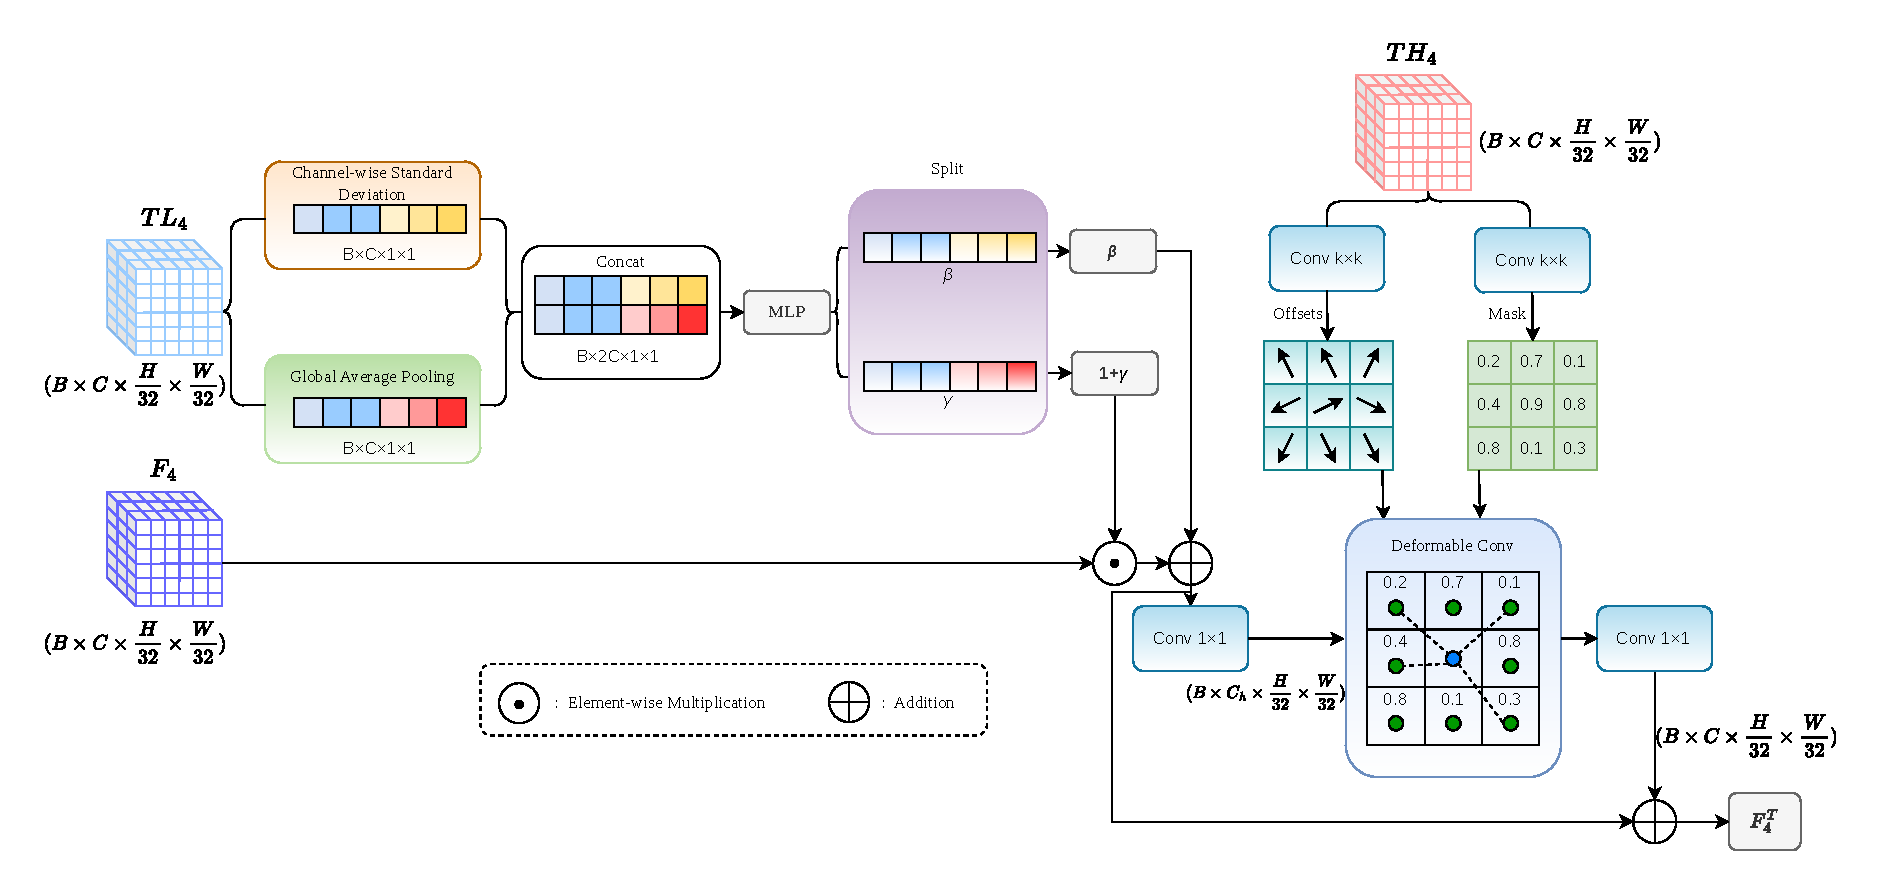
\includegraphics[width=1.0\textwidth]{tfrm.pdf}
  \caption{The detailed design of the proposed Temporal Frequency Reconfiguration Module (TFRM). The temporal low-frequency feature $\mathbf{T}^{L}_{4}$ generates channel-wise scaling and shifting parameters to modulate the single-frame frequency feature $\mathbf{F}_{4}$, while the temporal high-frequency feature $\mathbf{T}^{H}_{4}$ predicts offsets and modulation masks for deformable feature aggregation.}
  \label{fig:3}
  \vspace{-1em}
\end{figure*}

\vspace{-0.5em}
\subsection{ Temporal Frequency Reconfiguration Module}\label{TFRM}
To model temporal dynamics in video sequences, we employ the Temporal Discrete Wavelet Transform (DWT-T) to decompose two consecutive frames into a temporal low-frequency component and a temporal high-frequency component. The temporal low-frequency component captures slowly varying temporal trends and preserves the overall evolution of crowd distributions, whereas the temporal high-frequency component encodes rapid temporal variations and motion details between adjacent frames. Based on these temporal frequency characteristics, we design the temporal frequency reconfiguration module (TFRM) to inject temporal information into single-frame frequency features. Specifically, the temporal low-frequency feature is employed to generate FiLM-based\cite{perez2018film} scaling and shifting parameters for adaptive channel-wise modulation of the single-frame frequency feature, while temporal high-frequency cues guide DCNv2 \cite{zhu2019deformable} to dynamically adjust sampling locations for motion-aware feature aggregation.

Taking the TFRM at the scale of $\frac{H}{32} \times \frac{W}{32}$ for example, as shown in Fig.~\ref{fig:3}, the temporal low-frequency feature \(TL_4\) is first summarized using global average pooling and channel-wise standard deviation statistics to obtain \(z_{avg}\) and \(z_{std}\), respectively. The former captures the mean activation of each channel, while the latter describes the feature variation within each channel. These two descriptors are concatenated and fed into a shared multilayer perceptron (MLP) to generate adaptive modulation parameters, including a residual scaling factor $\boldsymbol{\gamma}$ and a bias term $\boldsymbol{\beta}$:
\begin{equation}
\begin{aligned}
\boldsymbol{\gamma}, \boldsymbol{\beta}
=
\operatorname{MLP}
\left(
\operatorname{Concat}
\left(
\mathbf{z}_{avg},
\mathbf{z}_{std}
\right)
\right).
\end{aligned}
\end{equation}
The generated parameters are applied to the single-frame frequency feature $F_4$ through a FiLM-based transformation:
\begin{equation}
\begin{aligned}
\hat{\mathbf{F}}
=
\left(1+\boldsymbol{\gamma}\right)
\odot
\mathbf{F_4}
+
\boldsymbol{\beta},
\end{aligned}
\end{equation}
To further enhance the spatial representation of the FiLM-modulated feature $\hat{\mathbf{F}}$, we employ temporal high-frequency cues to guide a deformable filtering process. To reduce the computational cost of deformable convolution, \(\hat{\mathbf{F}}\) is first projected to a lower-dimensional space using a \(1\times1\) convolution, followed by LayerNorm and GELU activation, yielding \(\mathbf{F}_{hidden}\). The temporal high-frequency feature $\mathbf{TH}_4$ is then used to predict adaptive sampling offsets and modulation masks, which guide the deformable filtering process:
\begin{equation}
\begin{aligned}
\Delta \mathbf{P}
&=
Conv_{k\times k}(\mathbf{TH}_4),
\\
\mathbf{M}
&=
\sigma(Conv_{k\times k}(\mathbf{TH}_4)),
\\
\hat{\mathbf{F}}_{hidden}
&=
DCN(\mathbf{F}_{hidden},\Delta \mathbf{P},\mathbf{M}),
\end{aligned}
\end{equation}
where $\Delta \mathbf{P}$ and $\mathbf{M}$ denote the learned sampling offsets and modulation masks, respectively, and $\sigma(\cdot)$ denotes the sigmoid activation function. Generated from the temporal high-frequency feature $\mathbf{TH}_4$, these parameters encode motion-sensitive cues and guide the deformable convolution to adaptively adjust its sampling patterns. As a result, $F_{hidden}$ can be spatially reconfigured to better capture dynamic crowd variations while preserving its underlying structural information.

Finally, $\hat{\mathbf{F}}_{\mathrm{hidden}}$ is projected back to the original channel dimension through a \(1\times1\) convolution, followed by LayerNorm and GELU activation. The resulting feature is then added to the modulated feature \(\hat{\mathbf{F}}\) through a residual connection to obtain the reconfigured frequency feature \(\mathbf{F}_4^{T}\). The refined feature \(\mathbf{F}_4^{T}\) simultaneously captures stable temporal context and dynamic motion information, providing a more discriminative frequency representation for subsequent feature interaction.


\begin{figure}
  \centering  
  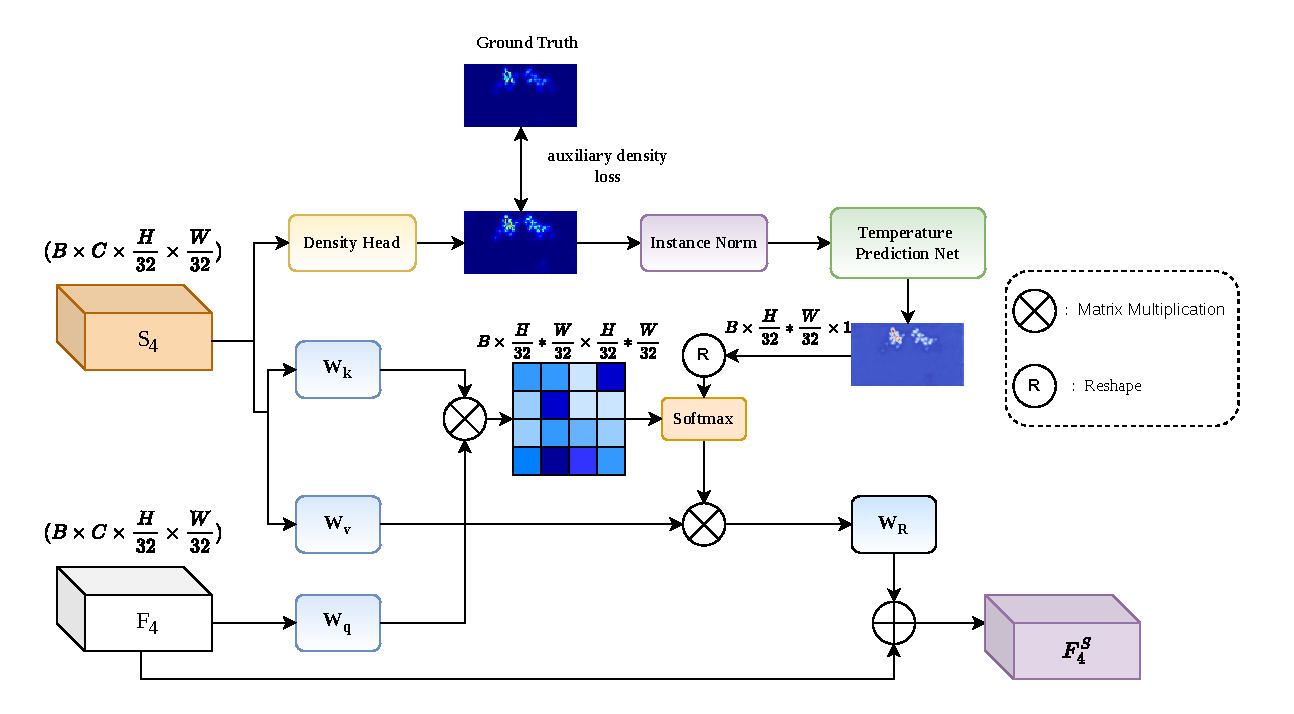
\includegraphics[width=0.48\textwidth]{dgfa.pdf}
  \caption{Architecture of the proposed Density-Guided Frequency Attention (DGFA) module at the $\frac{H}{32}\times\frac{W}{32}$ scale. The spatial feature $\mathbf{S}_{4}$ is used to estimate an auxiliary density map, which is further used to generate an adaptive temperature map for attention modulation. The frequency feature $\mathbf{F}_{4}$ serves as the query, while the key and value are projected from $\mathbf{S}_{4}$, producing the density-guided frequency representation $\mathbf{F}^{S}_{4}$.}
  \label{fig:4}
  \vspace{-1em}
\end{figure}
%, applied to feature $F_{target}$ using $F_{sourse}$
\vspace{-1em}

\subsection{Density-Guided Frequency Attention}\label{DGFA}
In the other branch, we introduce the density-guided frequency attention (DGFA) module to enhance the single-frame frequency representation $\mathbf{F}_4$ under the guidance of the fourth-stage spatial feature $\mathbf{S}_4$ extracted from the current frame. In DGFA, the spatial feature $\mathbf{S}_4$ is first used to predict a density map, which is subsequently fed into a lightweight temperature prediction network to generate an adaptive temperature map. The resulting temperature map dynamically modulates the attention distribution according to the crowd density, enabling more discriminative frequency feature enhancement.

As shown in Fig.~\ref{fig:4}, we first exploit the spatial feature \(\mathbf{S}_4\) to estimate a density map \(\mathbf{D}\), which serves as a crowd-distribution prior. To ensure the quality of the learned density prior, \(\mathbf{D}\) is supervised by the corresponding ground-truth density map using an auxiliary density loss, which will be introduced in Section~\ref{ls}. To capture relative density variations rather than absolute density values, \(\mathbf{D}\) is further normalized by instance normalization before being fed into the temperature prediction network. This operation is motivated by the fact that density maps usually contain many small-valued responses, which may lead the network to learn nearly uniform temperature values and weaken spatial adaptivity. By normalizing the density representation, we alleviate scale imbalance and facilitate the learning of adaptive temperature responses in the following temperature prediction network. 

Then, the normalized density map is fed into a lightweight temperature prediction network followed by a sigmoid activation to generate the adaptive temperature map \(\mathbf{T}\). Specifically, the network consists of two \(1\times1\) convolutional layers with a GELU activation, transforming the normalized density prior into adaptive temperature responses.

Next, the query is generated from $\mathbf{F}_4$, while the key and value are projected from $\mathbf{S}_4$. The attention computation is formulated as:
\begin{equation}
\mathbf{Q} = W_q(\mathbf{F}_4), \quad
\mathbf{K} = W_k(\mathbf{S}_4), \quad
\mathbf{V} = W_v(\mathbf{S}_4),
\end{equation}
\begin{equation}
\mathbf{A}
=
\mathrm{Softmax}
\left(
\frac{
\mathbf{Q}
\mathbf{K}^{\top}
\cdot s
}
{\mathbf{T}}
\right),
\end{equation}
\begin{equation}
\mathbf{F}_4^{S}
=
\mathbf{F}_4
+
W_R
\left(
\mathbf{A}\mathbf{V}
\right),
\end{equation}
where $\mathbf{Q}$, $\mathbf{K}$, and $\mathbf{V}$ denote the query, key and value, respectively, and $W_R(\cdot)$ represents the output projection. We empirically find that the conventional scaling factor \(1/\sqrt{d}\) may overly suppress the attention logits when combined with the adaptive temperature map \(\mathbf{T}\). Therefore, it is replaced by a learnable scale factor \(s\), which allows the attention scale to be fine-tuned during optimization. The output feature is projected to the original channel dimension and added to the input feature through a residual connection, yielding $\mathbf{F}^{S}_{4}$.

Thereafter, the proposed DGFA is further applied to the frequency features at the second scale of \(\frac{H}{16}\times\frac{W}{16}\). Under the guidance of density-aware spatial priors, the frequency features are refined to obtain \(\mathbf{F}_3^{S}\). By performing density-guided frequency enhancement at multiple feature scales, the model is able to capture crowd representations at multiple feature scales, thereby improving the discriminability of frequency features.

\begin{figure}
  \centering  
  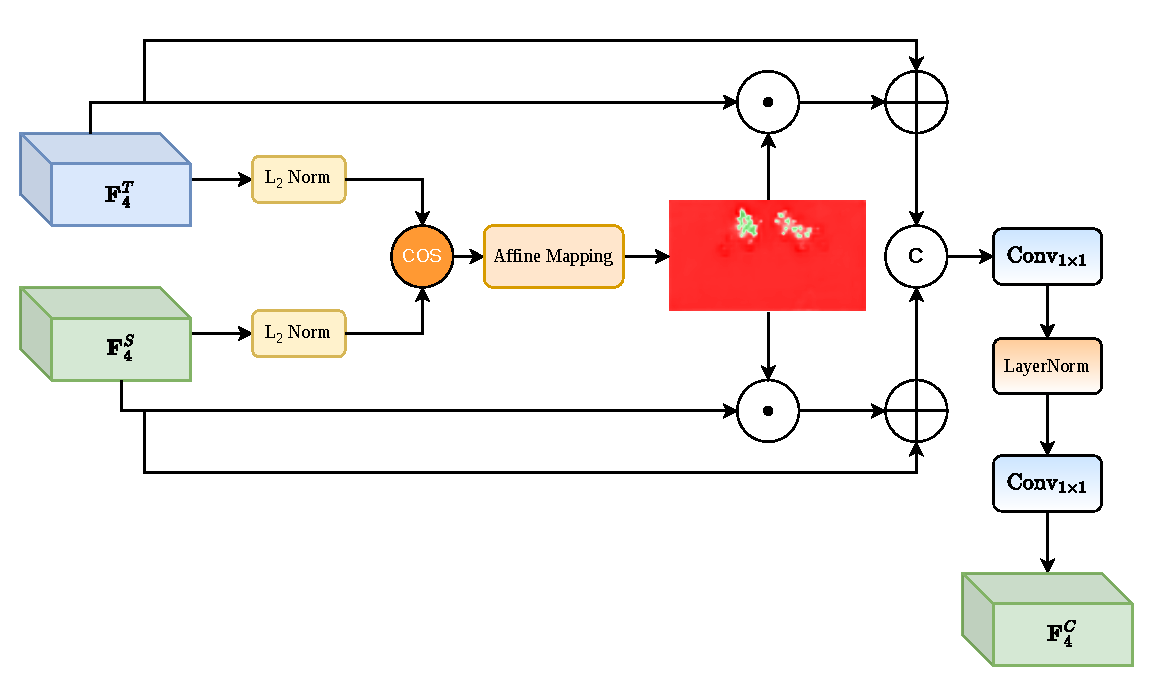
\includegraphics[width=0.48\textwidth]{DSE.pdf}
  \caption{The detailed design of the proposed Dual-Domain Similarity Enhancement (DSE) module. The temporal-frequency representation $\mathbf{F}^{T}_{4}$ and frequency-spatial representation $\mathbf{F}^{S}_{4}$ are first normalized to compute a pixel-wise cosine similarity map. The similarity map is then used to enhance semantically consistent regions in both representations, which are concatenated and projected to obtain the fused feature $\mathbf{F}^{C}_{4}$.}
  \label{fig:5}
  \vspace{-1em}
\end{figure}
\vspace{-1em}

%, followed by layer normalization
\subsection{Dual-Domain Similarity Enhancement Module} \label{fuse}
At the scale of $\frac{H}{32}\times\frac{W}{32}$, after obtaining the temporal-frequency representation $\mathbf{F}_4^{T}$ and the frequency-spatial representation $\mathbf{F}_4^{S}$, we propose a dual-domain similarity enhancement (DSE) module to fuse the information from the two branches. Instead of suppressing inconsistent responses through attention weighting, DSE explicitly amplifies spatial locations where the two representations exhibit high semantic consistency, allowing complementary information to be preserved while reinforcing reliable crowd cues. Inspired by CLRNet \cite{dong2022clrnet}, which models cross-locality relations via similarity reasoning for crowd representation learning, we introduce a cosine-similarity-based mechanism to measure the spatial consistency between $\mathbf{F}_4^{T}$ and $\mathbf{F}_4^{S}$. 

The spatial similarity map is computed by first performing channel-wise $\ell_2$ normalization and then calculating the cosine similarity at each spatial location:
\begin{equation}
\mathbf{M}_{raw}
=
\sum_{c=1}^{C}
\left(
\frac{\mathbf{F}_{4,c}^{T}}
{\|\mathbf{F}_4^{T}\|_2}
\odot
\frac{\mathbf{F}_{4,c}^{S}}
{\|\mathbf{F}_4^{S}\|_2}
\right),
\end{equation}

\begin{equation}
\mathbf{M}
=
\Phi
\left(
\mathbf{M}_{raw}
\right),
\end{equation}
where $\mathbf{M}_{raw}$ denotes the pixel-wise cosine similarity map and $\Phi(\cdot)$ denotes a fixed affine mapping that rescales the similarity values from $[-1,1]$ to $[0,1]$. Consequently, larger values in $\mathbf{M}$ indicate stronger semantic consistency between the temporal-frequency and frequency-spatial representations.

We employ the similarity map $\mathbf{M}$ to enhance semantically consistent regions while preserving complementary information from both branches:
\begin{equation}
\begin{aligned}
\hat{\mathbf{F}}_4^{T}
&=
\mathbf{F}_4^{T}
\odot
(1+\mathbf{M}),\\
\hat{\mathbf{F}}_4^{S}
&=
\mathbf{F}_4^{S}
\odot
(1+\mathbf{M}),
\end{aligned}
\end{equation}
where the factor $(1+\mathbf{M})$ adaptively strengthens spatial locations exhibiting high semantic consistency, while retaining all information from both branches. The enhanced features are concatenated and fused as:
\begin{equation}
\mathbf{F}_4^{C}
=
Conv_{1\times1}
\left(
LN
\left(
Conv_{1\times1}
\left(
\mathrm{Concat}
\left(
\hat{\mathbf{F}}_4^{T},
\hat{\mathbf{F}}_4^{S}
\right)
\right)
\right)
\right),
\end{equation}
The first 1×1 convolution compresses the concatenated features, while the second 1×1 convolution restores the channel dimension to obtain the fused representation $\mathbf{F}_4^{C}$. By enhancing semantically similar regions before fusion, DSE preserves complementary information from both branches and produces a more discriminative dual-domain representation. The same process is further applied at the scale of $\frac{H}{16}\times\frac{W}{16}$ to achieve multi-scale dual-domain feature fusion. Subsequently, the fused feature is projected to the $\frac{H}{8}\times\frac{W}{8}$ scale via a projection layer followed by bilinear interpolation, and then fed into the density head to generate the final density map prediction.



\subsection{Loss Function}\label{ls}
To train the proposed network, we adopt a density regression loss as the primary supervision and introduce auxiliary density loss and temporal consistency loss. The overall objective is formulated as:

\begin{equation}
\mathcal{L}
=
\mathcal{L}_{\mathrm{den}}
+
\lambda_a \mathcal{L}_{\mathrm{aux}}
+
\lambda_t \mathcal{L}_{\mathrm{temp}},
\end{equation}
where $\mathcal{L}_{\mathrm{den}}$ supervises the final density prediction, $\mathcal{L}_{\mathrm{aux}}$ provides direct supervision for the density priors learned in DGFA, and $\mathcal{L}_{\mathrm{temp}}$ encourages temporal consistency between consecutive density estimations. 

Given the predicted density map $\hat{D}_t$ and the ground-truth density map $D_t$ of frame $t$, the primary density regression loss is defined as:
\begin{equation}
\mathcal{L}_{\mathrm{den}}
=
\sum_{i=1}^{H}\sum_{j=1}^{W}
\left(
\hat{D}_t(i,j)-D_t(i,j)
\right)^2.
\end{equation}


As mentioned in Section\ref{DGFA}, DGFA predicts density maps from spatial features to provide density-aware priors for attention modulation. To ensure the quality of these learned density priors, we impose auxiliary supervision on the intermediate density maps generated at different feature stages. Let $\hat{D}_t^{s4}$ and $\hat{D}_t^{s3}$ denote the density maps predicted from the stage-4 and stage-3 spatial features, respectively. The auxiliary density loss is defined as

\begin{equation}
\mathcal{L}_{\mathrm{aux}}
=
\left\|
\hat{D}_t^{s4}
-
\mathcal{R}_{s4}(D_t)
\right\|_1
+
\left\|
\hat{D}_t^{s3}
-
\mathcal{R}_{s3}(D_t)
\right\|_1,
\end{equation}
where $\mathcal{R}_{s4}(\cdot)$ and $\mathcal{R}_{s3}(\cdot)$ denote bilinear resizing operations that align the ground-truth density map with the corresponding feature resolutions. By explicitly supervising these intermediate density maps, the network learns more reliable crowd-distribution priors, which further facilitate the density-guided attention mechanism.

Since the proposed framework adopts a frame-recurrent paradigm and explicitly exploits temporal frequency information, temporal consistency between adjacent predictions is further enforced through a temporal consistency loss. Given two consecutive frames $t-1$ and $t$, the predicted density variation and ground-truth density variation are computed as:

\begin{equation}
\Delta\hat{D}_t
=
\hat{D}_t-\hat{D}_{t-1},
\qquad
\Delta D_t
=
D_t-D_{t-1}.
\end{equation}
The temporal consistency loss is defined as:
\begin{equation}
\mathcal{L}_{\mathrm{temp}}
=
\frac{1}{HW}
\sum_{i=1}^{H}
\sum_{j=1}^{W}
\left|
\Delta\hat{D}_t(i,j)
-
\Delta D_t(i,j)
\right|.
\end{equation}
By matching the density variation between adjacent frames, $\mathcal{L}_{\mathrm{temp}}$ provides explicit supervision for temporal consistency. Consequently, the proposed objective jointly optimizes density estimation accuracy, density-prior quality, and temporal consistency in a unified manner.




\section{Experiments}
\subsection{Implementation Details}\label{ID}
During training, we follow MFA \cite{ling2023motional} and DACM \cite{ling2025dual} to perform data augmentation, including random cropping and horizontal flipping with a probability of $0.5$. For each dataset, the last 10\% of the training sequences are reserved for validation. The ConvNeXt-T\cite{liu2022convnet} and ConvNeXt-Atto\cite{woo2023convnext} are initialized with weights pre-trained on ImageNet-22K and ImageNet-1K, respectively. The network is optimized using AdamW with a weight decay of $1\times10^{-4}$. The learning rate is set to $5\times10^{-6}$ for all datasets except Venice~\cite{liu2019context}, where a larger learning rate of $1\times10^{-4}$ is adopted due to the extremely limited number of training samples. In the loss function, the hyperparameters $\lambda_a$ and $\lambda_t$ are both set to $1$. All experiments are implemented in PyTorch and conducted on an NVIDIA GeForce RTX 5090 GPU.



\vspace{-1em}
\subsection{Evaluation Metrics}
Experiments for evaluation are performed on five publicly available video crowd counting datasets (Bus \cite{ling2023motional}, Classroom \cite{ling2023motional}, Mall\cite{chen2012feature}, Venice \cite{liu2019context} and FDST \cite{fang2019locality}). Follow the convention of \cite{wu2022spatial,dong2022clrnet} and \cite{hou2023frame}, Mean Absolute Error (MAE) and Root Mean Squared Error (RMSE) are used to evaluate the counting performance of different methods, which are defined as follows:
\begin{equation}
\resizebox{.91\linewidth}{!}{$
            \displaystyle
\text{MAE}= \frac{1}{Z}\sum _{z=1}^{Z}|N_{z}^{gt}-N_{z}|,
\text{RMSE}= \sqrt{\frac{1}{Z}\sum _{z=1}^{Z}(N_{z}^{gt}-N_{z})^{2}},$}
\end{equation}
where $Z$ denotes the number of test frames, $N_{z}^{gt}$ and $N_{z}$ are the ground truth and the estimated count of $z$-th frame, respectively.


% \vspace{-1em}
\subsection{Comparison with the State-of-the-art Methods}

\begin{table}[h]
\caption{Comparisons with the state-of-the-art methods on Bus and Classroom. The best result is emphasized as \textbf{bold} and the second-best is represented as \underline{underlined}}
\centering
\scriptsize
\begin{tabular}{cccccc}
    \toprule
    \multirow{2}{*}{Category}&Dataset&\multicolumn{2}{c}{Bus}&\multicolumn{2}{c}{Classroom}\\
    &Method &MAE & RMSE&MAE & RMSE\\
    \midrule
     %& CSRNet \cite{li2018csrnet} & 1.99 & 2.40 & 3.42 & 3.86 \\
   Image & CAN \cite{liu2019context} & 2.25 & 2.69 & 1.72 & 2.09 \\
   & Bayesian \cite{ma2019bayesian} &3.03 & 3.70 & 2.86 & 3.14 \\
   & RR \cite{wan2019residual} &  1.67 & 2.03 & 4.07 & 4.38 \\
   & KDMG \cite{wan2020kernel} &  2.43 & 2.92 & 4.17 & 4.48 \\
   & DMCount \cite{wang2020distribution} & 2.37 & 2.95 & 2.86 & 3.49 \\
   & TopoCount \cite{abousamra2021localization}  & 2.69 & 3.44 & 2.75 & 3.34 \\
   & P2PNet \cite{song2021rethinking}  & 4.28 & 5.26 & 1.63 & 2.08 \\ 
   & MAN \cite{lin2022boosting} & 2.75 & 3.28 & 2.35 & 2.72 \\ 
   & ConvNeXt \cite{liu2022convnet}  & 1.65 & 2.01 & 3.17 & 3.93 \\
   & CHS-Net \cite{dai2023cross} & 1.81 & 2.19 & 1.46 & 1.80 \\
   & HMoDE \cite{du2023redesigning} & 1.77 & 2.13 & 1.49 & 1.95 \\  
   & Gramformer \cite{lin2024gramformer}  & 2.25 & 2.62 & 1.65 & 2.07 \\  
   \midrule
   Video & LSTN \cite{fang2019locality} &  2.47 & 3.13 & 3.02 & 3.90 \\
   & EPF \cite{liu2020estimating} & 1.69 & 2.08 & 2.16 & 2.48 \\
   & STGN \cite{wu2022spatial} & 1.58 & 1.92 & 1.54 & 1.83 \\
   & MFA \cite{ling2023motional} & 1.42 & 1.80 & 1.64 & 2.00 \\ 
   & DACM \cite{ling2025dual} & \underline{1.32} & \textbf{1.66} & 1.70 & 2.03 \\ 
   & DSTI \cite{ling2026dual} & \underline{1.32} & \underline{1.68} & \underline{1.42} & \underline{1.71}  \\
   & WaveLoop  & \textbf{1.30} & \textbf{1.66} & \textbf{1.30} & \textbf{1.54} \\
    \bottomrule
\end{tabular}
\label{tab:1}
 \vspace{-1em}
\end{table}


\textit{1) Bus and Classroom}:
The Bus and Classroom datasets~\cite{ling2023motional} are two challenging indoor video crowd counting benchmarks. As shown in Table~\ref{tab:1}, the proposed WaveLoop achieves the best performance on both datasets among 12 image-based and 6 video-based methods. Compared with image-based approaches, WaveLoop outperforms all compared image-based methods on both datasets. Specifically, on the Bus dataset, WaveLoop reduces the MAE and RMSE by 21.2\% and 17.4\%, respectively, compared with ConvNeXt~\cite{liu2022convnet}, the best image-based baseline on this dataset. On the Classroom dataset, WaveLoop surpasses CHS-Net~\cite{dai2023cross}, the best-performing image-based method, by 11.0\% in MAE and 14.4\% in RMSE.

The proposed WaveLoop also demonstrates competitive advantages over video-based methods. On the Bus dataset, the proposed WaveLoop obtains an MAE/RMSE of 1.30/1.66, achieving the best MAE and a competitive RMSE among video-based methods. Compared to the suboptimal DACM~\cite{ling2025dual}, WaveLoop reduces MAE by 1.5\% while maintaining comparable RMSE performance. On the Classroom dataset, the proposed WaveLoop surpasses DSTI\cite{ling2026dual} by 8.5\% in MAE and 9.9\% in RMSE. These improvements can be attributed to the proposed temporal-frequency recurrent counting framework. The temporal frequency reconfiguration module (TFRM) exploits the complementary characteristics of low- and high-frequency temporal components to enhance temporal representations and reduce frame-wise count fluctuations. Furthermore, the density-guided frequency attention (DGFA) facilitates effective information exchange between spatial and frequency-domain features, leading to more discriminative feature fusion and improved robustness in challenging indoor scenes. By incorporating recurrent propagation of historical density estimates and jointly modeling spatial, temporal, and frequency information, WaveLoop achieves more accurate and temporally stable crowd counting results.



\begin{table}[h]
\caption{Comparisons with the state-of-the-art methods on FDST}
\centering
\scriptsize
\begin{tabular}{@{}cccc@{}}
\toprule
Category & Method & MAE & RMSE  \\ 
\midrule
 %& CSRNet \cite{li2018csrnet} & 2.56 & 3.12 \\
Image & Bayesian \cite{ma2019bayesian} & 2.85 & 3.74 \\
& CAN \cite{liu2019context} & 2.44 & 2.96 \\
& ADCrowdNet \cite{liu2019adcrowdnet} & 2.18 & 2.84 \\
& RPNet \cite{yang2020reverse} & 2.38 & 3.03 \\
& Gramformer \cite{lin2024gramformer} & 5.15 & 6.32 \\
\midrule
 %& Bi-ConvLSTM \cite{xiong2017spatiotemporal}  & 4.48 & 5.82 \\
Video & LSTN \cite{fang2019locality} & 3.35 & 4.45 \\
& EPF \cite{liu2020estimating} & 2.10 & 2.46 \\
& MOPN \cite{hossain2020video}  & 1.76 & 2.25 \\
& PHNet \cite{meng2021phnet} & 1.65 & 2.16 \\
& GNANet \cite{li2022video} & 2.10 & 2.90 \\
& GRGAF-ST \cite{cai2022global} & 1.91 & 2.45 \\
& CLRNet \cite{dong2022clrnet} & 1.45 & 1.97 \\
& MFA* \cite{ling2023motional} & 1.90 & 2.60 \\
& FRVCC \cite{hou2023frame} & 1.62 & 2.36 \\
& STGN \cite{wu2022spatial} & {1.38} & {1.82} \\
& SSCR \cite{yong2025lightweight} & 2.06 & 2.53 \\
& DACM \cite{ling2025dual} & 1.31 & 1.75 \\
& E-MAC \cite{cao2024efficient} & 1.29 & 1.69 \\
& DSTI \cite{ling2026dual} & 1.33 & 1.71 \\
& CCINet \cite{ling2026cascaded} & \underline{1.25} & \textbf{1.62} \\
& WaveLoop  & \textbf{1.16} & \underline{1.64} \\
\bottomrule
\end{tabular}
\label{tab:2}
 \vspace{-1em}
\end{table}

\textit{2) FDST} \cite{fang2019locality}:
As a large-scale video crowd counting benchmark with diverse indoor and outdoor scenes, FDST poses significant challenges to the robustness and generalization ability of counting models. As shown in Table~\ref{tab:2}, the proposed WaveLoop outperforms 5 image-based and 14 video-based methods. Notably, MFA* results~\cite{ling2023motional} in the table are regenerated using official code with resized images (640 $\times$ 360) for fair comparison. Compared with the strongest image-based method ADCrowdNet~\cite{liu2019adcrowdnet}, WaveLoop achieves substantial improvements, reducing the MAE and RMSE by 46.8\% and 42.3\%, respectively. Compared with the recent state-of-the-art video-based method CCINet~\cite{ling2026cascaded}, WaveLoop further reduces the MAE by 7.2\%, while maintaining a competitive RMSE. These results indicate that the proposed framework can more effectively exploit temporal dependencies and cross-domain complementary information, thereby producing more accurate and robust density estimation in complex scenes.

For qualitative evaluation, Figure~\ref{fig:6} presents the visualization results of WaveLoop on the FDST dataset, including both outdoor (a–b) and indoor (c–d) scenes. The predicted density maps closely match the corresponding ground-truth distributions, indicating that the proposed method can accurately estimate both the spatial distribution and density of crowds. In outdoor scenes, WaveLoop effectively captures people distributed over large areas while maintaining clear responses in densely populated regions. In indoor environments with cluttered backgrounds and severe occlusions, WaveLoop still produces density maps that closely match the ground truth, with high-density regions accurately localized. These qualitative results demonstrate that the proposed method generalizes well across diverse crowd scenes and is capable of producing reliable density estimation under different environmental conditions.

%For qualitative comparison, Fig.~\ref{fig:6} visualizes the counting results of WaveLoop and the recent video-based method CCINet~\cite{ling2026cascaded} on FDST. Compared with CCINet, WaveLoop produces density maps that better align with the underlying crowd distribution and yields predictions closer to the ground truth. In particular, it can preserve clearer responses in crowded regions while suppressing irrelevant background interference, leading to more reliable counting performance under severe occlusion and complex scene layouts. These visual results are consistent with the quantitative comparisons in Table~\ref{tab:2}, further demonstrating the effectiveness of the proposed method on challenging video crowd counting scenarios.


\begin{figure*}[t]
\centering

\subfloat[]{
    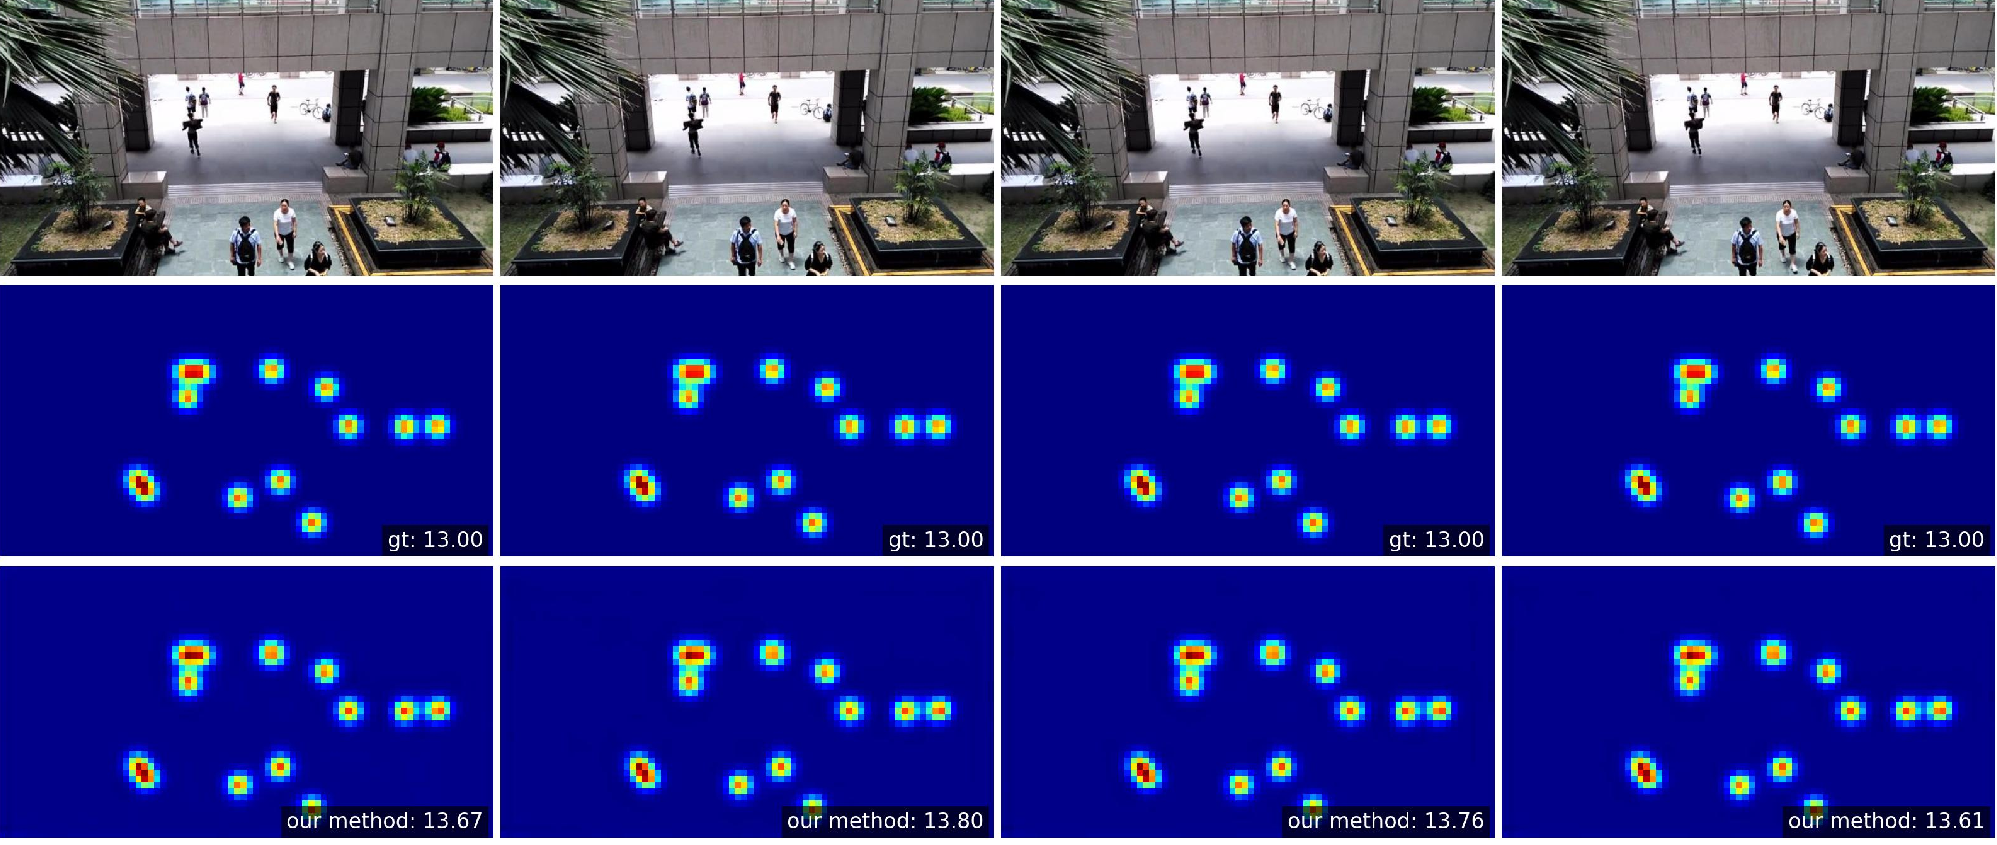
\includegraphics[width=0.47\textwidth]{outdoor1.pdf}}
\hfill
\subfloat[]{
    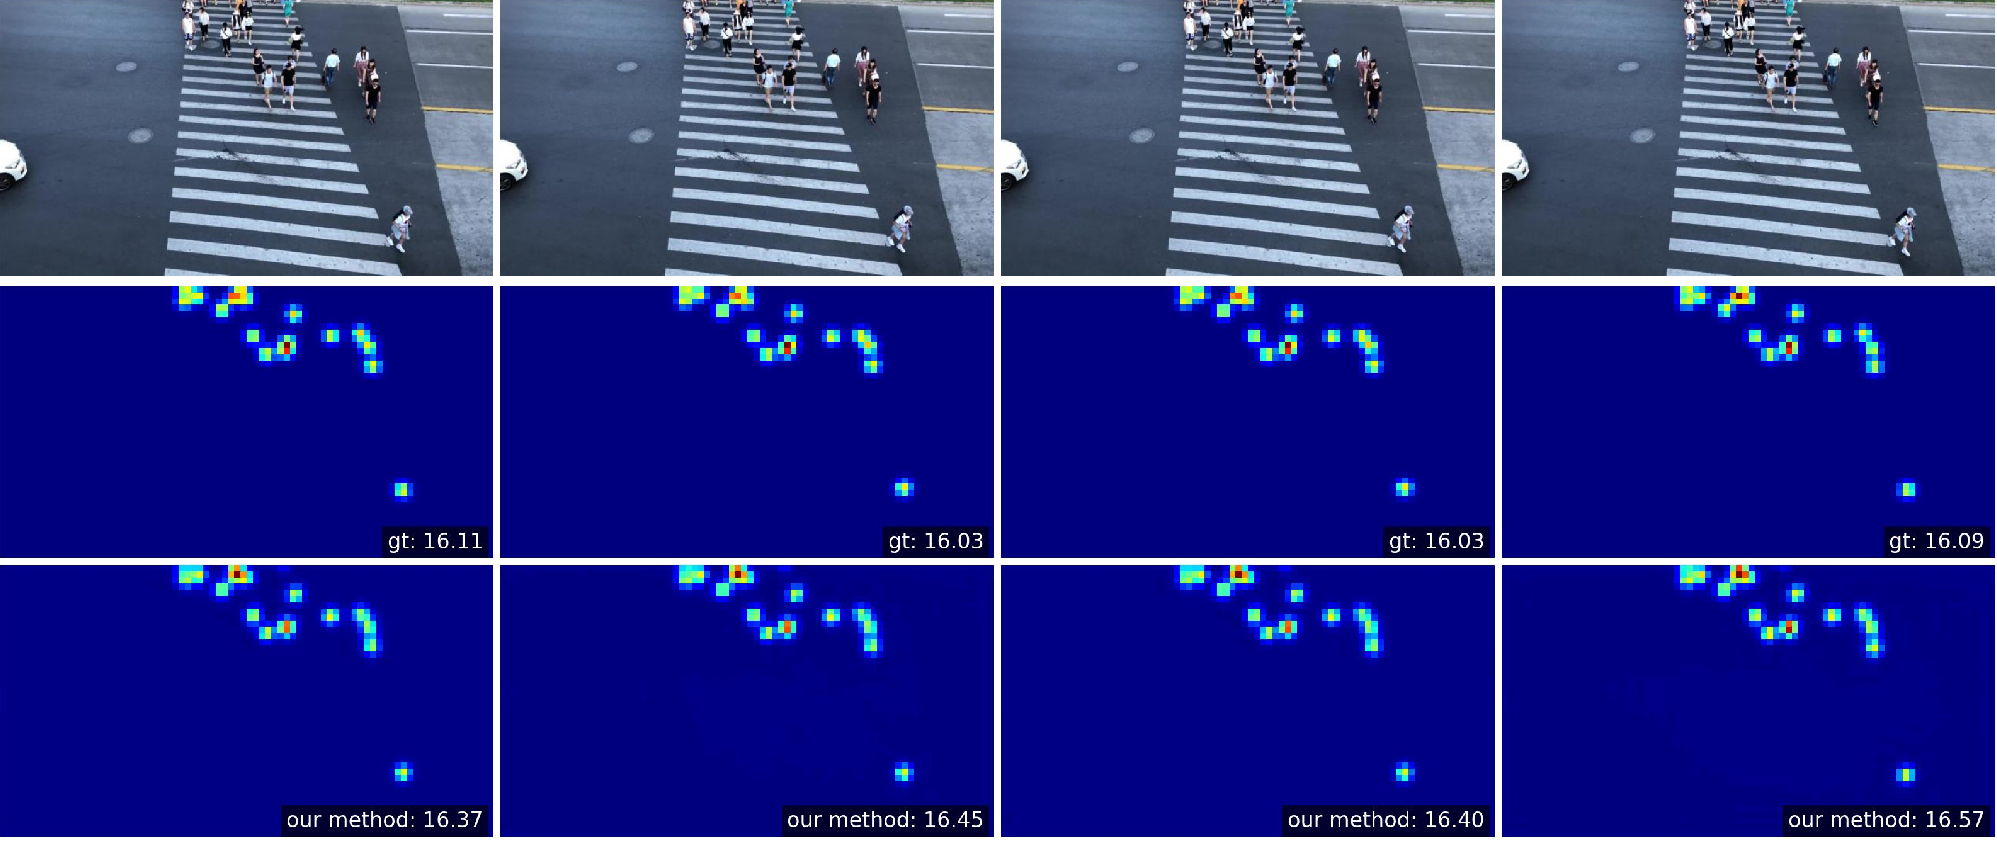
\includegraphics[width=0.47\textwidth]{outdoor2.pdf}}
\\[0.2em]

\subfloat[]{
    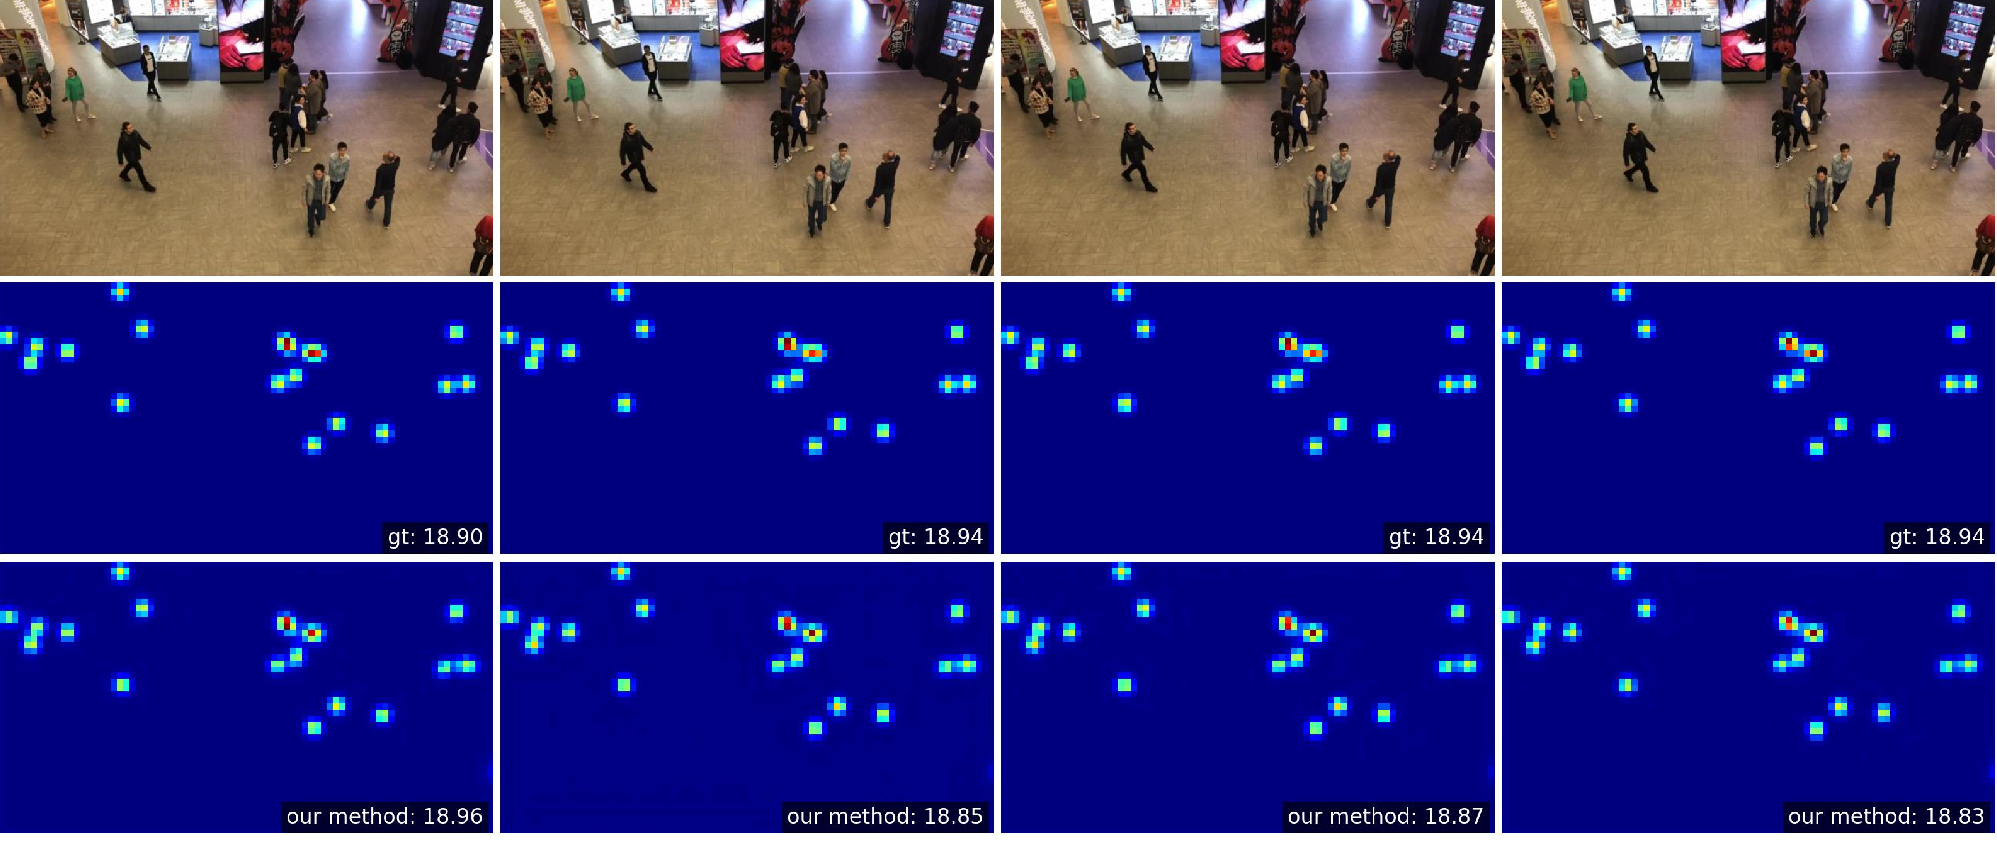
\includegraphics[width=0.47\textwidth]{indoor1.pdf}}
\hfill
\subfloat[]{
    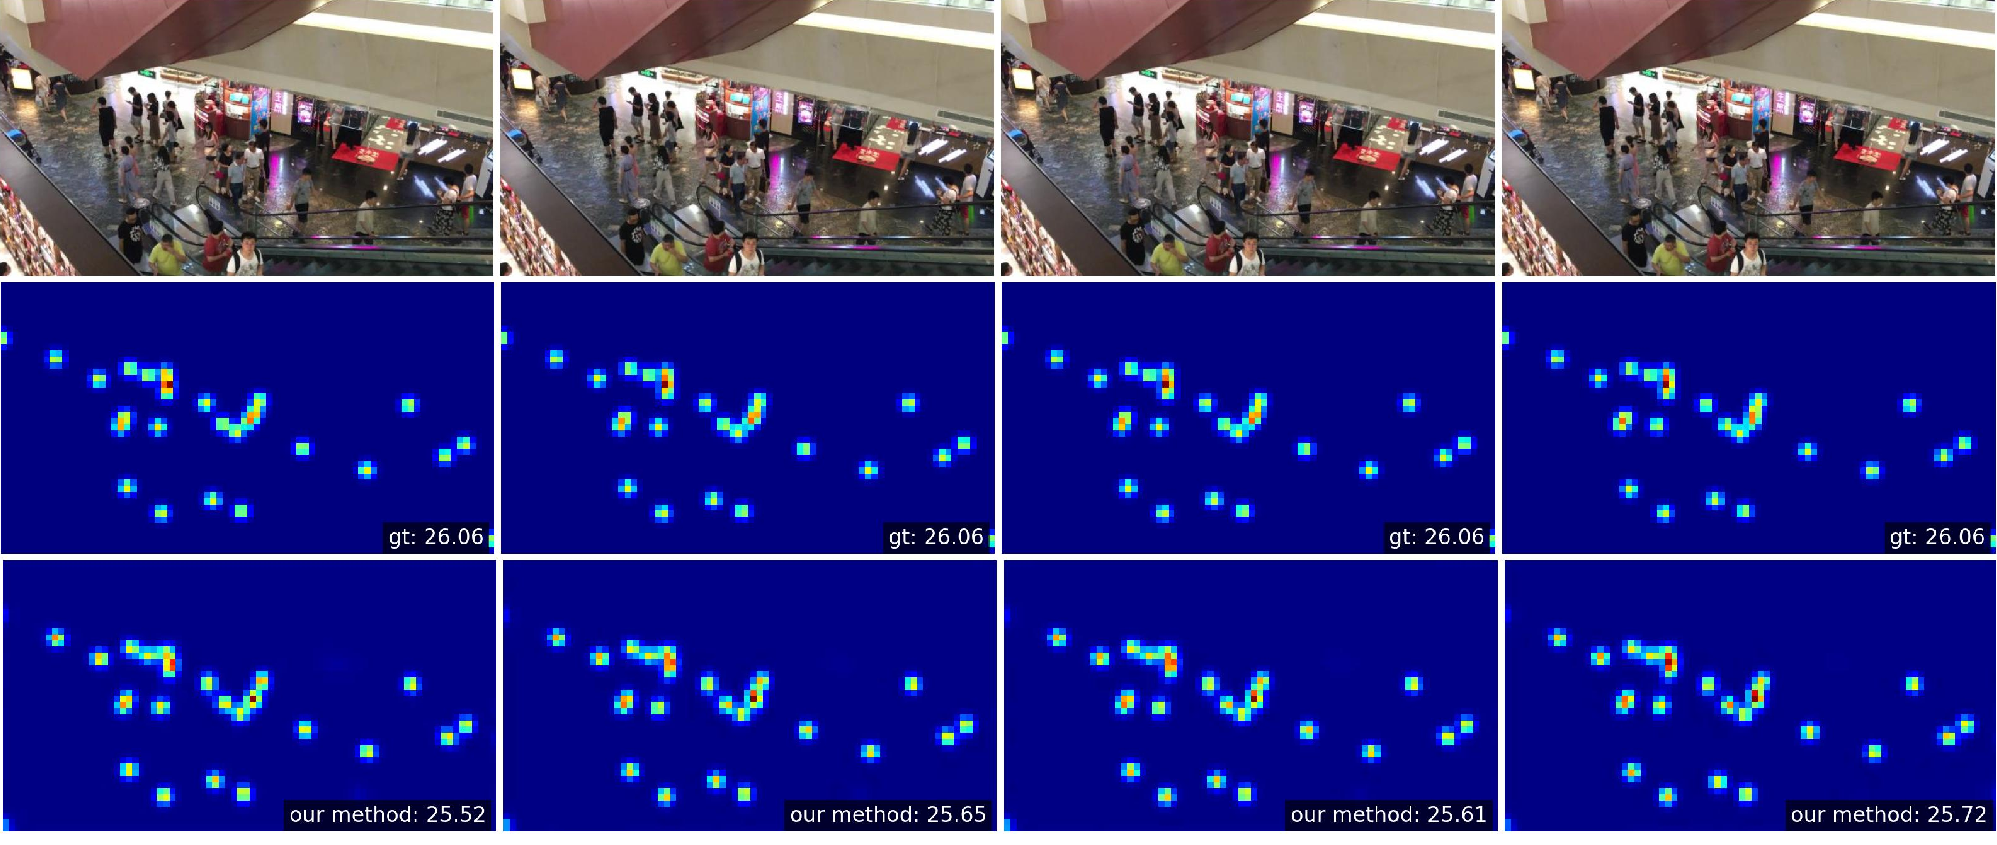
\includegraphics[width=0.47\textwidth]{indoor2.pdf}}

\caption{Visualized comparisons on the FDST dataset. The first row shows the input frames, the second row presents the corresponding ground-truth density maps, and the third row shows the density maps predicted by WaveLoop.}
\label{fig:6}
\vspace{-1em}
\end{figure*}

\begin{table}[h]
\caption{Comparisons with the state-of-the-art methods on Mall}
\centering
\scriptsize
\begin{tabular}{@{}cccc@{}}
\toprule
Category & Method & MAE & RMSE  \\ 
\midrule
Image & RR \cite{wan2019residual}  & 2.52 & 3.09 \\
& Bayesian \cite{ma2019bayesian}  & 1.96 & 2.49 \\ 
& ADCrowdNet \cite{liu2019adcrowdnet}  & 1.92 & 2.45 \\
& KDMG \cite{wan2020kernel}  & 2.35 & 2.92 \\
& RPNet \cite{yang2020reverse}  & 2.20 & 3.60 \\
& DMCount \cite{wang2020distribution}  & 2.02 & 2.52 \\
& MAN \cite{lin2022boosting}  & 2.14 & 2.71 \\
& ConvNeXt \cite{liu2022convnet}  & 1.62 & 2.02 \\
& CHS-Net \cite{dai2023cross}  & 1.71 & 2.18 \\
& HMoDE \cite{du2023redesigning}  & 1.70 & 2.14 \\
& Gramformer \cite{lin2024gramformer}  & 1.69 & 2.14 \\
\midrule
Video & LSTN \cite{fang2019locality}  &2.00 & 2.50 \\
& E3D \cite{zou2019enhanced}  & 1.64 & 2.13 \\
& MOPN \cite{hossain2020video}  & 1.78 & 2.25 \\
& GRGAF-ST \cite{cai2022global}  &1.61 & 2.07 \\
& STGN \cite{wu2022spatial}  & 1.53 & 1.97 \\
& MFA \cite{ling2023motional}  & 1.51 & 1.93 \\
& DACM \cite{ling2025dual}  & \underline{1.44} & \underline{1.85} \\
& DSTI \cite{ling2026dual}  & 1.51 & 1.92 \\
& WaveLoop & \textbf{1.36}& \textbf{1.71}\\
\bottomrule
\end{tabular}
\label{tab:3}
\vspace{-1em}
\end{table}

\textit{3) Mall} \cite{chen2012feature}:
Mall is a widely used benchmark for video crowd counting, containing complex pedestrian distributions and frequent occlusions in indoor scenes. As shown in Table~\ref{tab:3}, the proposed WaveLoop is compared with 11 image-based methods and 8 video-based methods, and achieves the best performance on both metrics, with an MAE of \textbf{1.36} and an RMSE of \textbf{1.71}. Compared with the strongest image-based method ConvNeXt~\cite{liu2022convnet}, WaveLoop reduces the MAE and RMSE by 16.0\% and 15.3\%, respectively. This result indicates that exploiting temporal dependencies across consecutive frames is more effective than relying solely on spatial appearance for crowd estimation in surveillance videos.

Compared with the recent state-of-the-art video-based method DACM~\cite{ling2025dual}, WaveLoop further reduces the MAE and RMSE by 5.6\% and 7.6\%, respectively. Such improvements demonstrate the effectiveness of the proposed recurrent cross-domain modeling strategy for Mall, where crowd distributions vary continuously across adjacent frames. By jointly leveraging temporal-frequency cues and spatial representations, WaveLoop can produce more accurate and stable density estimations, thereby achieving superior performance over previous video crowd counting methods.



\begin{table}[h]
\caption{Comparisons with the state-of-the-art methods on Venice}
\centering
\scriptsize
\begin{tabular}{@{}cccc@{}}
\toprule
Category & Method & MAE & RMSE  \\ 
\midrule
 %& CSRNet \cite{li2018csrnet} & 35.8 & 50.0 \\
Image & ADCrowdNet \cite{liu2019adcrowdnet} & 24.2 & 40.1 \\
& CAN \cite{liu2019context} & 23.5 & 38.9 \\
& ECAN \cite{liu2019context} & 20.5 & 29.9 \\
& RPNet \cite{yang2020reverse} & 26.3 & 43.3 \\
& Gramformer \cite{lin2024gramformer} & 21.3 & 28.6 \\
%& EHNET \cite{yan2025ehnet} & 22.4 & 32.2 \\
\midrule
Video & EPF \cite{liu2020estimating} & 15.0 & 19.6 \\
& PHNet \cite{meng2021phnet} & 18.1 & 25.1 \\
& STGN \cite{wu2022spatial} & 14.1 & 20.1 \\
& FRVCC \cite{hou2023frame}  & {13.2} & {16.5} \\
& DACM \cite{ling2025dual} & \underline{11.1} & \underline{14.3} \\
& DSTI \cite{ling2026dual} & 11.6 & 14.8 \\
& WaveLoop  & \textbf{10.4} & \textbf{14.2} \\
\bottomrule
\end{tabular}
\label{tab:4}
\vspace{-1em}
\end{table}

\textit{4) Venice} \cite{liu2019context}:
The Venice dataset is particularly challenging due to its very limited training set and the large viewpoint differences between training and testing sequences. As shown in Table~\ref{tab:4}, the proposed WaveLoop achieves the best overall performance on the Venice dataset, surpassing all 5 image-based methods and 6 video-based methods. Compared with the strongest image-based method Gramformer~\cite{lin2024gramformer}, WaveLoop reduces the MAE and RMSE by 51.2\% and 50.3\%, respectively. These results suggest that, for small-scale datasets such as Venice, incorporating temporal information is highly beneficial for improving the robustness and accuracy of crowd estimation under large scene variations.

Compared with the recent video-based method DACM~\cite{ling2025dual}, WaveLoop further reduces the MAE by 6.3\% and the RMSE by 0.7\%. We attribute this improvement mainly to the proposed scale-aligned frequency fusion (SAFF) module. Specifically, SAFF adaptively rescales the high-frequency components according to the statistical magnitude of the low-frequency component before aggregation, which alleviates the mismatch in value range between different frequency bands and enables more effective frequency-domain feature fusion. This design is particularly beneficial for Venice, where the limited training data and significant viewpoint shifts make robust representation learning more difficult. By preserving complementary high-frequency details while maintaining stable low-frequency structural information, SAFF helps the model produce more reliable density estimations in challenging scenes.



\vspace{-1em}
\subsection{Ablation Study}
\subsubsection{Component Analysis}
\noindent
To validate the effectiveness of each component in WaveLoop, we conduct an ablation study on the Classroom dataset, as presented in Table~\ref{tab:5}. We start with the ConvNeXt-T baseline, which yields an MAE of 1.93 and an RMSE of 2.32. By introducing the proposed SAFF module, the MAE/RMSE are reduced by 17.1\%/19.4\% with only 0.6M additional parameters, demonstrating that SAFF effectively leverages the complementary advantages of global low-frequency representations and local high-frequency details. Subsequently, incorporating the TFRM further improves the MAE/RMSE by 2.5\%/4.3\%, indicating that temporal frequency modeling effectively captures temporal dependencies and enhances temporal consistency across adjacent frames. 

Furthermore, integrating the proposed DGFA module further decreases the MAE/RMSE by 3.2\%/3.4\%, verifying that density-guided cross-domain interaction facilitates more effective feature fusion between the spatial and frequency domains. Finally, after incorporating the DSE module, the complete WaveLoop achieves the best performance with an MAE of 1.30 and an RMSE of 1.54, further reducing the MAE/RMSE by 13.9\%/11.0\% while introducing only 0.2M additional parameters. Overall, WaveLoop achieves improvements of 32.6\% and 33.6\% over the baseline. These results demonstrate that enhancing the consistent regions during dual-branch feature fusion is beneficial for video crowd counting, leading to more discriminative feature representations and more accurate density estimation.



\begin{table}[h]
\caption{Ablation Study of WaveLoop Components on Classroom}
  \centering
\scriptsize
\setlength{\tabcolsep}{3pt}
    \begin{tabular}[]{cccccccc}
    \toprule
   Baseline & SAFF & TFRM & DGFA & DSE & MAE & RMSE & Parameters (M) \\
    \midrule
    \checkmark &  &  &  &  & 1.93 & 2.32 & 28.0 \\
    \checkmark & \checkmark &  &  &  & 1.60 & 1.87 & 28.6 \\
    \checkmark & \checkmark & \checkmark &  &  & 1.56 & 1.79 & 39.3 \\
    \checkmark & \checkmark & \checkmark & \checkmark &  & 1.51 & 1.73 & 41.7 \\
    \checkmark & \checkmark & \checkmark & \checkmark & \checkmark & \textbf{1.30} & \textbf{1.54} &  41.9 \\ 
    \bottomrule
    \end{tabular}
\label{tab:5}
\vspace{-1em}
\end{table}

\subsubsection{Effect of Loss Weights}
To investigate the influence of the two auxiliary loss weights, we independently vary the temporal consistency loss weight $\lambda_t$ and the auxiliary density loss weight $\lambda_a$ while fixing the other weight to 1. Specifically, when evaluating $\lambda_t$, $\lambda_a$ is fixed at 1, and vice versa. The loss weights are selected from ${0,0.5,1.0,1.5,2.0}$, and the corresponding results are summarized in Table~\ref{tab:6}.

As shown in Table~\ref{tab:6}, the temporal consistency loss weight $\lambda_t$ achieves the best performance when set to 1.0. Removing the temporal consistency constraint ($\lambda_t=0$) or assigning an excessively large weight ($\lambda_t>1.0$) both lead to inferior performance, indicating that an appropriate temporal consistency constraint is beneficial for stable optimization. For the auxiliary density loss weight $\lambda_a$, the best performance is also achieved at $\lambda_a=1.0$, while both insufficient and excessive auxiliary supervision degrade the counting accuracy. Therefore, setting $\lambda_t=\lambda_a=1.0$ provides the best balance between the auxiliary objectives and the primary density regression task, yielding the lowest MAE of 1.30 and RMSE of 1.54.


\begin{table}[h]
\centering
\caption{Effect of loss weights on Classroom}
\begin{tabular}{cccccc}
\toprule
Parameter & 0 & 0.5 & 1.0 & 1.5 & 2.0 \\
\midrule
$\lambda_t$ (MAE)  & 1.58 & 1.52 & \textbf{1.30} & 1.37 & 1.62 \\
$\lambda_t$ (RMSE) & 1.79 & 1.83 & \textbf{1.54} & 1.63 & 1.94 \\
\midrule
$\lambda_a$ (MAE)  & 1.54 & 1.59 & \textbf{1.30} & 1.62 & 1.74 \\
$\lambda_a$ (RMSE) & 1.75 & 1.99 & \textbf{1.54} & 1.91 & 1.94 \\
\bottomrule
\end{tabular}
\label{tab:6}
\end{table}






\subsubsection{Transfer learning}
Transfer learning experiments are conducted to evaluate the generalization capability of the proposed WaveLoop. Following previous works~\cite{xiong2017spatiotemporal,ling2023motional,ling2025dual}, the experiments are performed on the UCSD and Mall datasets, which exhibit substantial differences in scene layouts, crowd densities, and frame rates. Specifically, all training images from the source domain are first used to train the model. Following the convention of MFA~\cite{ling2023motional}, after the source-domain training is completed, 50 images from the target domain are selected to fine-tune the model using a small learning rate of $1\times10^{-6}$. We compare WaveLoop with four non-deep-learning-based approaches (LGP, FA, GPA, and GPTL), two image-based methods (MCNN and CSRNet), and four video-based crowd counting methods (Bi-ConvLSTM, MOPN, DACM and CCINet). The quantitative results are summarized in Table~\ref{tab:7}. For the UCSD $\rightarrow$ Mall task, WaveLoop achieves the second-best result with an MAE of 2.44, only 0.08 higher than the best-performing MOPN\cite{hossain2020video}. For the Mall $\rightarrow$ UCSD task, WaveLoop obtains the best result with an MAE of 1.53, outperforming the previous state-of-the-art MOPN by 1.3\%. These results demonstrate that the proposed WaveLoop exhibits strong generalization capability across datasets with different scene characteristics and effectively transfers the learned representations to unseen domains.




\begin{table}[h]
\caption{Quantitative results of transfer learning using the UCSD and Mall datasets. The best result is emphasized as \textbf{bold} and the second-best is represented as \underline{underlined}}
  \centering
\scriptsize
    \begin{tabular}[]{ccc}
    \toprule
    Method & UCSD $\rightarrow$ Mall & Mall $\rightarrow$ UCSD  \\
     & MAE & MAE  \\
    \midrule
    LGP \cite{yu2005learning} & 4.36 & 3.32  \\     
    FA \cite{change2013semi} & 7.47 & 4.44 \\ 
    GPA \cite{liu2015bayesian} & 4.18 & 2.79  \\  
    GPTL \cite{liu2015bayesian} & 3.55 & 2.91  \\
    MCNN \cite{zhang2016single} & 24.25 & 11.26  \\
    Bi-ConvLSTM \cite{xiong2017spatiotemporal} & 2.63 & 1.82  \\
    CSRNet \cite{li2018csrnet} & 14.01 & 13.96 \\ 
    MOPN \cite{hossain2020video} & \textbf{2.36} & \underline{1.55} \\
    DACM \cite{ling2025dual} & 2.49 & 1.78 \\
    CCINet \cite{ling2026cascaded} & 2.45 &  1.65 \\
    \midrule
    WaveLoop & \underline{2.44} &  \textbf{1.53} \\
    \bottomrule
    \end{tabular}
\label{tab:7}
\vspace{-1em}
\end{table}


\subsubsection{Complexity Study}
In Table~\ref{tab:8}, we report the number of parameters, GFLOPs, inference time, and  performance on the Bus dataset for comparison with three representative methods. The GFLOPs are computed on two consecutive input frames with a resolution of $384\times384$, and the inference time is calculated for 100 images with 1024 × 1024 resolution on an NVIDIA RTX 4090 GPU. Compared with the recent video-based method MFA~\cite{ling2023motional}, WaveLoop reduces the parameter count from 58.63M to 41.94M while achieving the best counting accuracy, with MAE and RMSE reduced by 8.5\% and 7.8\%, respectively. The higher computational cost mainly stems from two aspects. First, WaveLoop jointly encodes single-frame features from the current frame and temporal frequency features decomposed into low- and high-frequency components, leading to additional feature extraction. Second, the proposed density-guided frequency attention (DGFA) is applied at two feature scales to facilitate spatial-frequency interaction, which further increases the computational complexity. Despite the additional overhead, these designs substantially improve the representation capability and result in more accurate crowd counting. Further improving the computational efficiency of the recurrent framework while maintaining its counting accuracy will be investigated in future work.


\begin{table}[h]
\caption{Complexity Study. P represents Parameters (M), IT denotes Inference Times (s) and MAE/RMSE are reported on the Bus dataset}
  \centering
\scriptsize
    \begin{tabular}[]{ccccccc}
    \toprule
    Category & Method & P & GFLOPs & IT  & MAE & RMSE\\
    \midrule    
    Image & Bayesian \cite{ma2019bayesian} & \textbf{21.50} & 60.73 & 6.19 & 3.03 & 3.70\\  
     &  MAN \cite{lin2022boosting} & 30.96 & 59.54 & 6.92 & 2.75 & 3.28\\  
    \midrule
     %Video & STGN\cite{wu2022spatial} & \textbf{12.55} & 51.02 & 4.11 & 1.38 & 1.82\\
     & MFA \cite{ling2023motional} & 58.63 & \textbf{55.01} & \textbf{5.23}  & 1.42 & 1.80\\ 
     & WaveLoop  & 41.94 & 64.99 & 7.09 & \textbf{1.30} & \textbf{1.66} \\
    \bottomrule
    \end{tabular}
\label{tab:8}
\vspace{-1em}
\end{table}

\subsubsection{Effect of kernel size in the TFRM on Classroom}
We investigate the effect of kernel size in the TFRM. As shown in Table~\ref{tab:8}, the best performance is achieved with a $3\times3$ kernel, obtaining an MAE/RMSE of 1.30/1.54. Reducing the kernel size to $1\times1$ increases the MAE and RMSE by 11.5\% and 11.0\%, respectively, indicating that local neighborhood information is important for temporal feature modeling. Although larger kernels provide wider receptive fields, the $5\times5$ and $7\times7$ kernels still result in performance degradation, with MAE/RMSE increases of 2.3\%/3.2\% and 6.9\%/7.1\%, respectively. This suggests that excessively large receptive fields may introduce irrelevant contextual information and weaken local temporal-frequency modeling. Therefore, a $3\times3$ kernel is adopted as the default setting in TFRM.





\begin{table}[h]
\caption{Effect of kernel size in the TFRM on Classroom}
  \centering
  \scriptsize
    \begin{tabular}[]{ccc}
    \toprule
    Kernel Size & MAE & RMSE\\
    \midrule    
    $1\times1$ & 1.45 & 1.71\\
    $3\times3$ & \textbf{1.30} & \textbf{1.54}\\
    $5\times5$ & 1.33 & 1.59\\
    $7\times7$ & 1.39 & 1.65\\
    \bottomrule
    \end{tabular}
\label{tab:9}
\vspace{-1em}
\end{table}



\subsubsection{Effect of Learning Rate and Weight Decay}
We further investigate the influence of the learning rate and weight decay on the performance of the proposed WaveLoop on the Classroom dataset. As shown in Fig.~\ref{fig:7}(a) and (b), the best performance, in terms of both MAE and RMSE, is achieved with a learning rate of $5\times10^{-6}$ and a weight decay of $1\times10^{-4}$. Either increasing or decreasing these hyperparameters results in inferior performance, demonstrating that appropriate optimization settings are crucial for achieving optimal counting accuracy.


\begin{figure}[h]
\centering
\subfloat[]{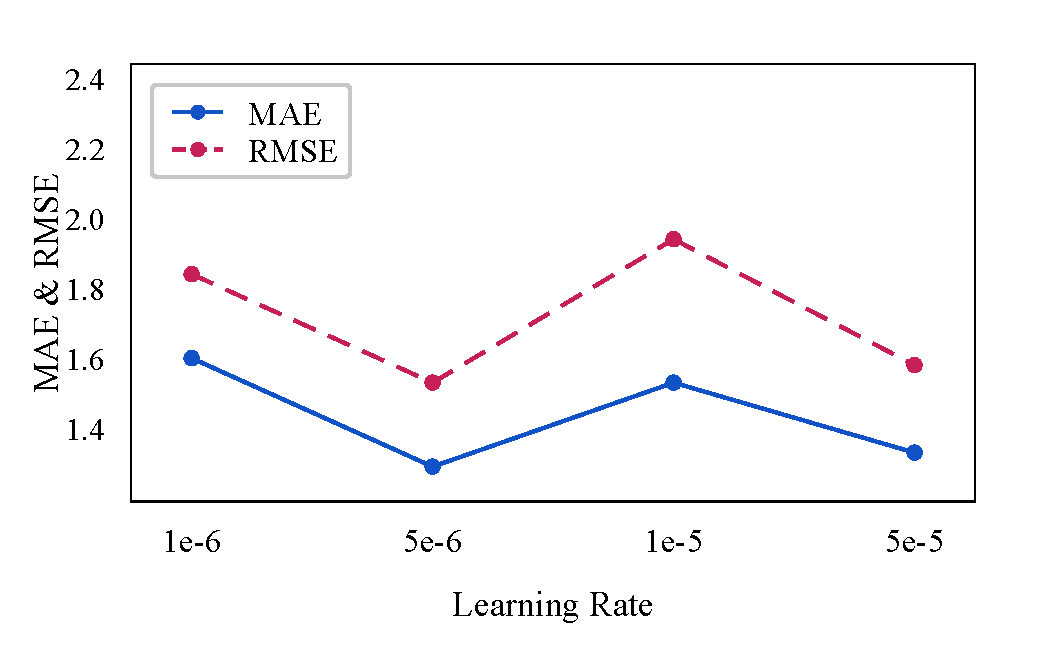
\includegraphics[height=0.31\linewidth]{lr.pdf}}
  \hfill
  \subfloat[]{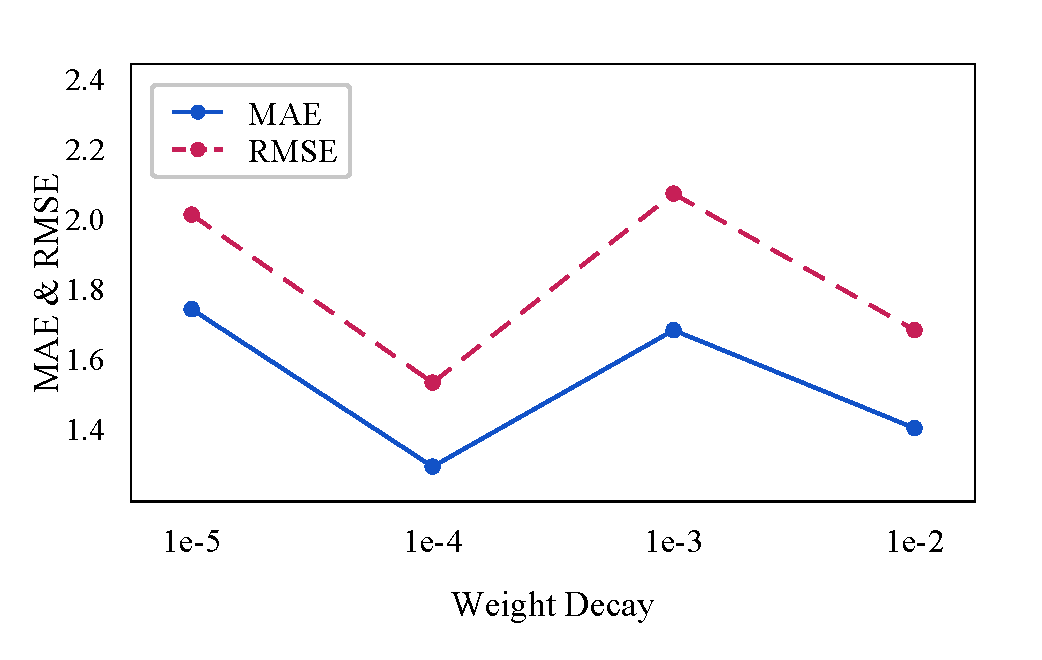
\includegraphics[height=0.31\linewidth]{decay.pdf}}
  \caption{Effect of (a) learning rate and (b) weight decay on Classroom.}
  \label{fig:7}
   \vspace{-1em}
\end{figure}





\section{Discussion and Conclusions}
In this paper, we presented WaveLoop, a frame-recurrent wavelet network for video crowd counting. WaveLoop models temporal variations through temporal discrete wavelet transform and recurrently propagates historical density predictions across frames. The proposed SAFF module reduces the magnitude discrepancy between spatial frequency bands, while the TFRM injects temporal information into single-frame frequency features. In addition, the DGFA module introduces density-aware spatial guidance for frequency enhancement, and the DSE module reinforces consistent responses between temporal-frequency and frequency-spatial representations. A temporal consistency loss is further employed to constrain density variations across adjacent frames. Experiments on five benchmark datasets show that WaveLoop achieves competitive or state-of-the-art performance, while the ablation studies verify the contribution of each component.

Despite its counting accuracy, WaveLoop introduces additional computation because spatial features and temporal-frequency representations are encoded jointly, and density-guided attention is applied at multiple feature scales. Therefore, reducing the computational cost of the recurrent framework remains an important direction for future work. Another possible extension is to investigate more robust temporal-frequency representations for scenes with abrupt motion, severe illumination changes, and rapidly varying crowd distributions.

\bibliographystyle{IEEEtran} 
\bibliography{refs.bib}



\begin{IEEEbiography}[{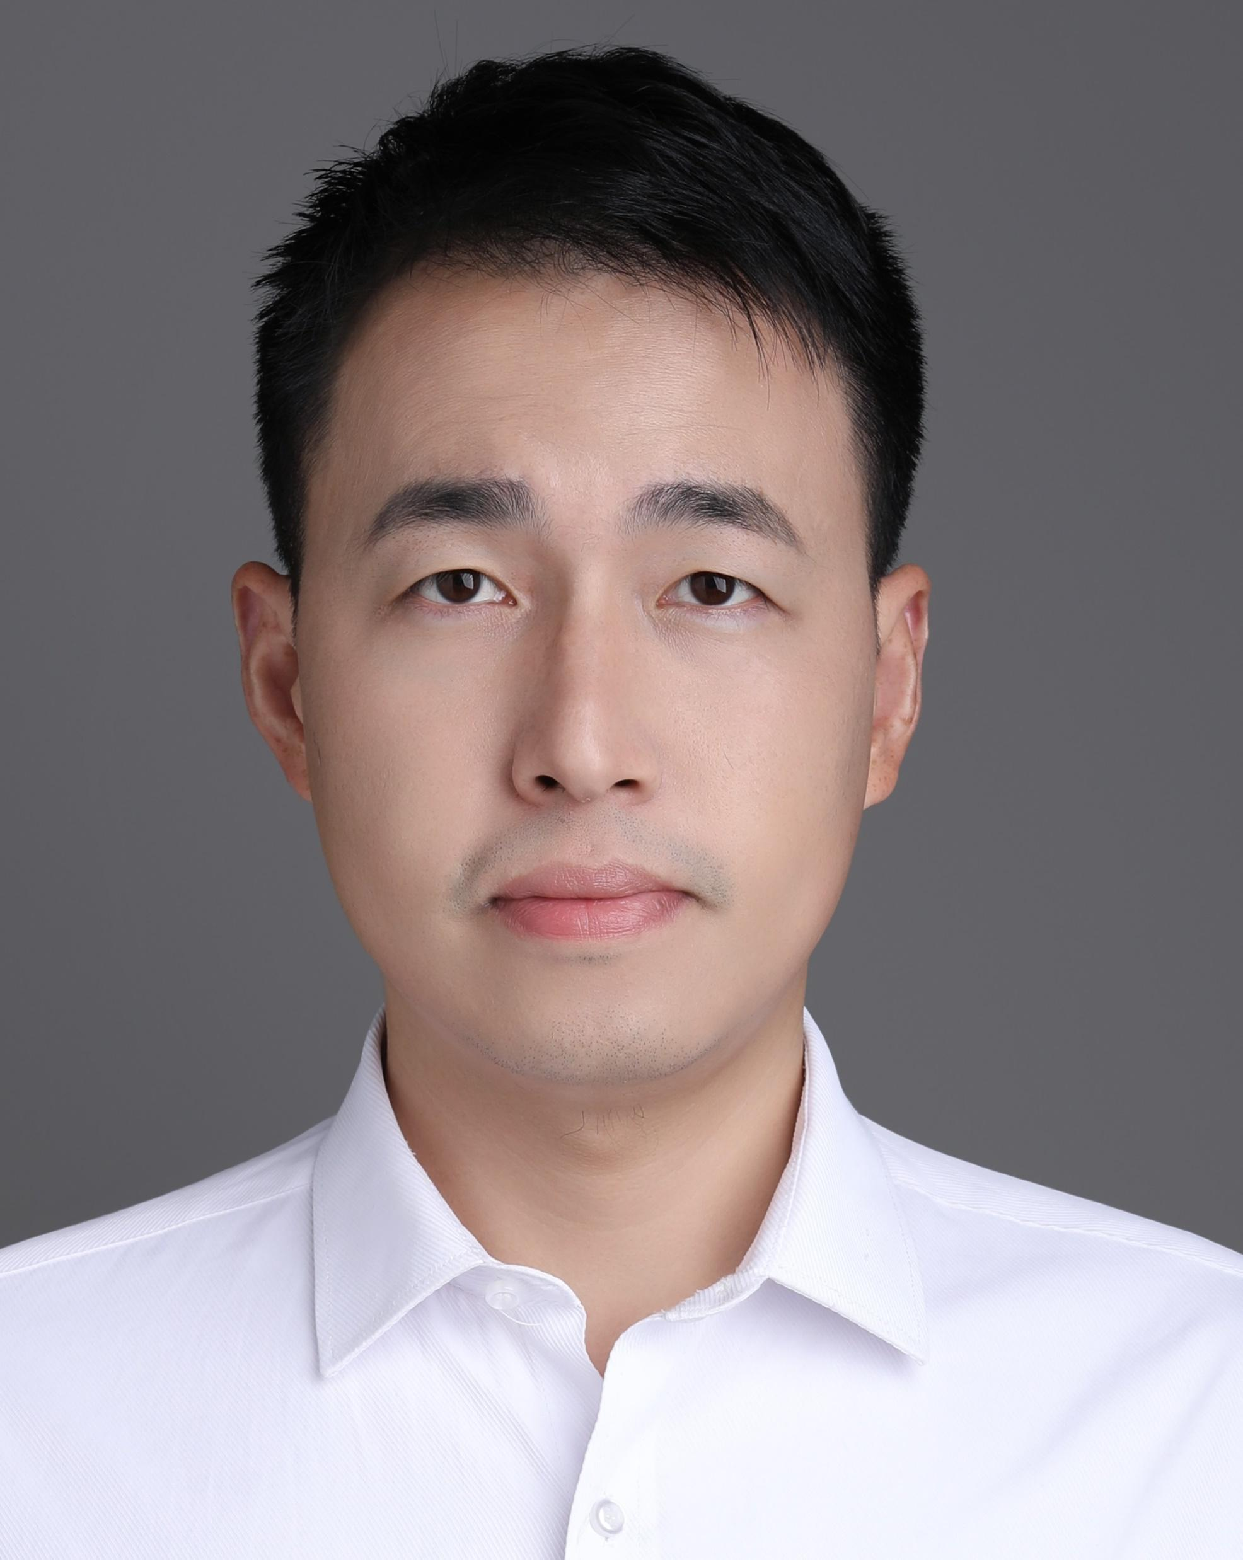
\includegraphics[width=1in,height=1.25in,clip,keepaspectratio]{ling.pdf}}]{Miaogen Ling} is currently an associate professor at Nanjing University of Information Science and Technology, China. He received the B.S. (2010) degree in mathematical science from the Soochow University, China and the M.S. degree and the Ph.D (2019) degree in computer science from the Southeast University, China. His research interests include deep learning and its application to computer vision and multimedia analysis.
\end{IEEEbiography}

\vspace{-3em}

\begin{IEEEbiography}
[{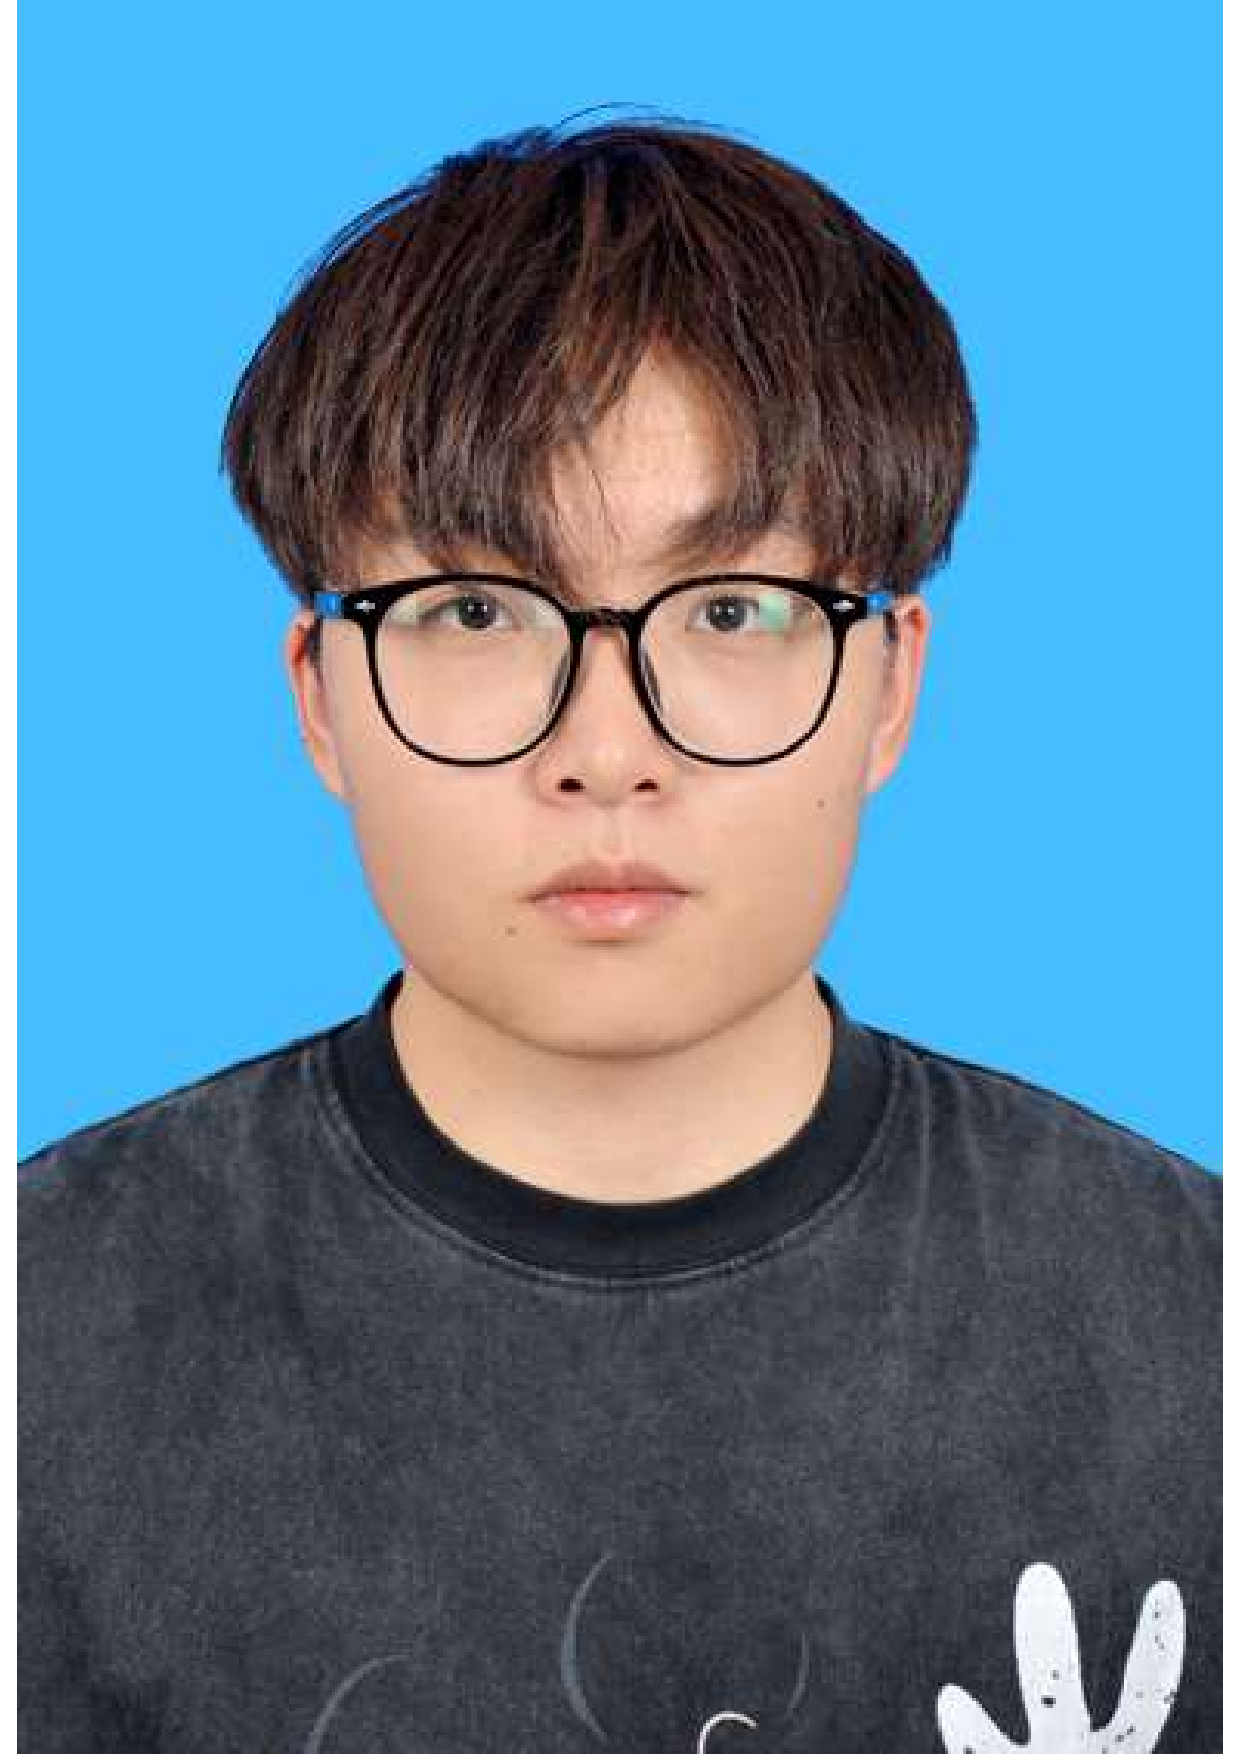
\includegraphics[width=1in,height=1.25in,clip]{sun.pdf}}]{Junyu Sun}
is currently pursuing the M.S. degree in Computer Science and Technology at Nanjing University of Information Science and Technology, China. He received the B.S. degree in Computer Science and Technology from SanJiang University, China, in 2024. His research interests include deep learning and its applications in computer vision.
\end{IEEEbiography}

\vspace{-3em}

\begin{IEEEbiography}
[{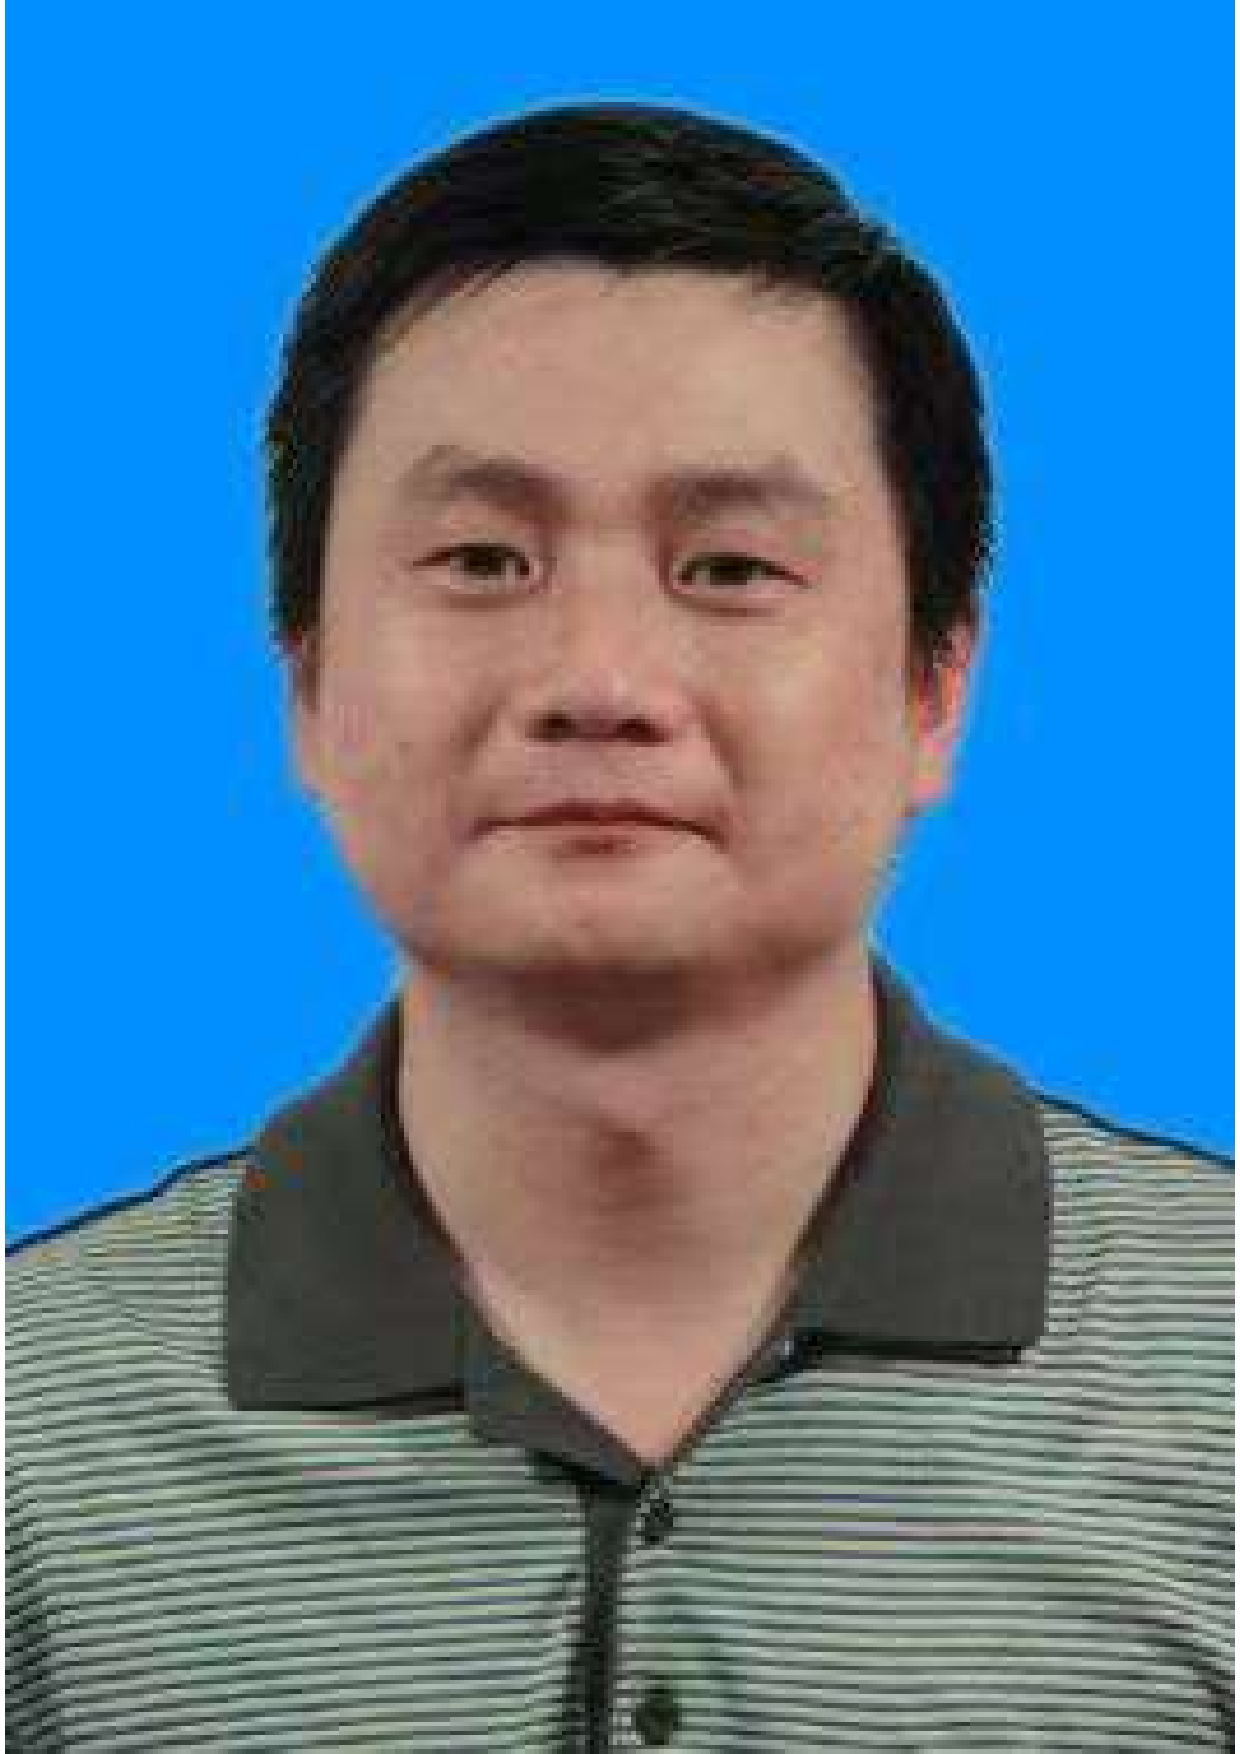
\includegraphics[width=1in,height=1.25in,clip]{fang.pdf}}]{Wei Fang} received the M.Sc. and Ph.D. degrees in computer science from Soochow University, Suzhou, China. He is currently a Professor with Jiangsu Engineering Center of Network Monitoring, Nanjing University of Information Science and Technology, Nanjing, China, State Key Laboratory for Novel Software Technology, Nanjing University, Nanjing. His research interests are in the areas of artificial
intelligence, big data analysis of meteorology, deep learning and cloud computing. Dr. Fang is a PC member for a number of international conferences and a reviewer for several international journals.
\end{IEEEbiography}

\vspace{-3em}

\begin{IEEEbiography}
[{
\includegraphics[width=1in,height=1.25in,clip,keepaspectratio]{geng.pdf}}]{Xin Geng} (Senior Member, IEEE) is a chair professor of Southeast University, China. His research interests include machine learning, pattern recognition, and computer vision. He has published over 100 refereed papers in these areas. He has been an Associate Editor of IEEE T-MM, FCS and MFC, a Steering Committee Member of PRICAI, a Program Committee Chair for conferences such as PRICAI’18, VALSE’13, etc., an Area Chair for conferences such as IJCAI, CVPR, ACMMM, ICPR, and a Senior Program Committee Member for conferences such as IJCAI, AAAI, ECAI, etc. He is a Distinguished Fellow of IETI and a Senior Member of IEEE.
\end{IEEEbiography}

\vfill

\end{document}


